\chapter{局部平坦性、协变微分与曲率}

\lectureoverview{度规总可以通过一阶近似在一个选定点处化为欧几里得形式。曲率始于这种坐标自由终结之处：即相邻局部标架无法彼此吻合的二阶失效。我们分三个阶段展开这一陈述。首先是法坐标，然后是协变导数及其联络，最后是两个协变导数的非对易性，它定义了黎曼张量，并赋予潮汐引力以不变量意义。}

\section{指标的必然负担}

广义相对论以一种相当特殊的方式显得困难。它的基本思想并非难以理解，但计算很快就会挤满指标、导数和符号。存在更紧凑的语言：vielbein、微分形式、旋量、twistor 以及相关工具，可以把冗长的分量方程打包成紧凑的对象。然而，学习这些语言本身就是一项繁重的任务，而且紧凑的记号可能掩盖初次接触时最需要理解的机制。

麦克斯韦方程组提供了范例。逐分量写出时，它们相当于若干个独立的方程。矢量记号把它们汇集为散度和旋度方程，使结构更易于看出。广义相对论也有类似的压缩方式，但当必须真正进行显式计算时，分量方法仍然是可靠的途径。因此我们将让指标保持可见。一旦熟悉了它们的语法，概念路径就会顺畅得多，尽管算术仍可能写满许多页。

符号计算软件包可以帮助处理这些算术。给定度规 \(g_{mn}(x)\)，这样的软件包可以构造克里斯托费尔符号、黎曼张量、里奇张量和爱因斯坦张量。然后它可以把这些表达式代入场方程。这并没有消除理解这些对象含义的必要性。它只是把机械展开与几何分离开来。

\begin{classroomqa}
\audiencequestion{在这次讲座之时，广义相对论有哪些活跃的研究领域？}
\lecturerresponse{讲座特别指出了若干前沿。量子引力与黑洞的量子物理是基础理论中的核心问题。经典天体物理与数值相对论研究诸如轨道运动并合的黑洞等系统，在这些系统中，求解爱因斯坦方程并预言引力辐射远不只是把方程盲目地喂给计算机。同样的数学结构也在凝聚态物理和流体动力学中找到用途。历史性的要点同样引人注目：广义相对论已经从 1960 年代一个相对较小的专门领域，转变为理论物理的核心语言之一，并与量子场论紧密相连。
\lecturetimestamp{00:05:15}}
\end{classroomqa}

这是最后一讲专门讨论黎曼几何本身。从下一讲开始，几何将被解释为引力。桥梁已经可见。区分真实的引力场与由加速坐标或曲线坐标引起的表观场，在数学上与区分弯曲度规和用别扭坐标写出的平坦度规是同一个问题。

\section{不变量问题}

当欧几里得几何在内在意义上成立时，二维几何就是平坦的：直线、平行线、三角形关系和距离测量都具有其欧几里得形式。人们容易说平坦意味着
\(g_{mn}=\delta_{mn}\)，但这一陈述依赖于坐标。即便是普通平面，在极坐标中也有依赖于位置的度规。正确的陈述是：一个平坦区域容许这样的坐标，使得度规在该区域中处处为常值且为欧几里得形式。

反之，假设度规以某种任意坐标交到我们手中。一个糟糕的检验方法是逐个搜索坐标系，每次都变换度规，并希望最终找到笛卡儿形式。可能性有无穷多个，所以这不是一个实用的判据。

正确的策略是从 \(g_{mn}\) 及其导数构造一个诊断量。我们想要一个对象 \(R\)，它具有两个决定性的性质：
\[
\begin{aligned}
R=0
&\quad\Longleftrightarrow\quad
\text{locally flat geometry},\\
R\neq 0 \text{ at } P
&\quad\Longrightarrow\quad
\text{curvature at } P.
\end{aligned}
\]
最重要的是，\(R\) 必须是一个张量。在一个坐标系中为零的张量在每个坐标系中都为零，因此不需要搜索坐标。

\begin{figure}[H]
\centering
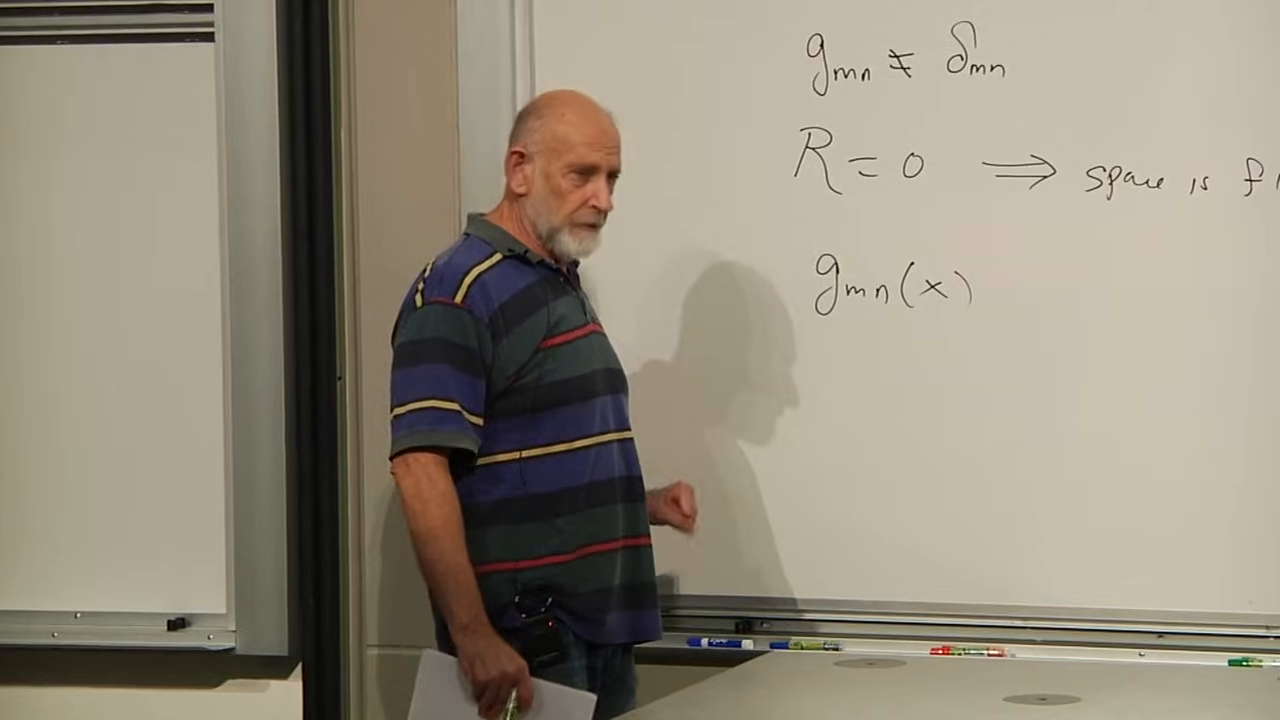
\includegraphics[width=\linewidth]{lecture_03_figure_01.png}
\caption{所期望的不变量检验：度规不必在表面上等于 \(\delta_{mn}\)，而一个为零的曲率对象应当标识出局部平坦的几何。}
\lectureframe{00:18:20}
\end{figure}

\emph{局部地}这一限定很重要。黎曼张量消失保证了局部欧几里得几何；但整体的等同仍可能产生非平凡的拓扑。例如，平坦的圆柱面或平坦的环面可以局部是欧几里得的，而整体上并不是平面。

\section{小尺度下的度规几何}

看看随维度变化会发生什么是有帮助的。零维空间只是一个点。连通的二维黎曼空间可以局部拉直成一条直线；整体上它可能是一条线段、一条直线或一个环。一只被限制在闭合一维轨道上的虫子可以测量其周长，但把轨道在外部房间中弯曲并不会改变其内禀度规。

二维允许丰富得多的内禀几何：平面、球面、凹凸不平的地球表面和环面即使在局部也未必一致，它们的整体拓扑也可以不同。度规是记录其无穷小距离的工具：
\begin{equation}
 ds^2=g_{mn}(x)\,dx^m dx^n.
\label{eq:l3-line-element}
\end{equation}
量\(ds^2\)是一个标量。因此，\(dx^m\)在坐标变换下的变化恰好被\(g_{mn}\)的变换所补偿。

\begin{figure}[H]
\centering
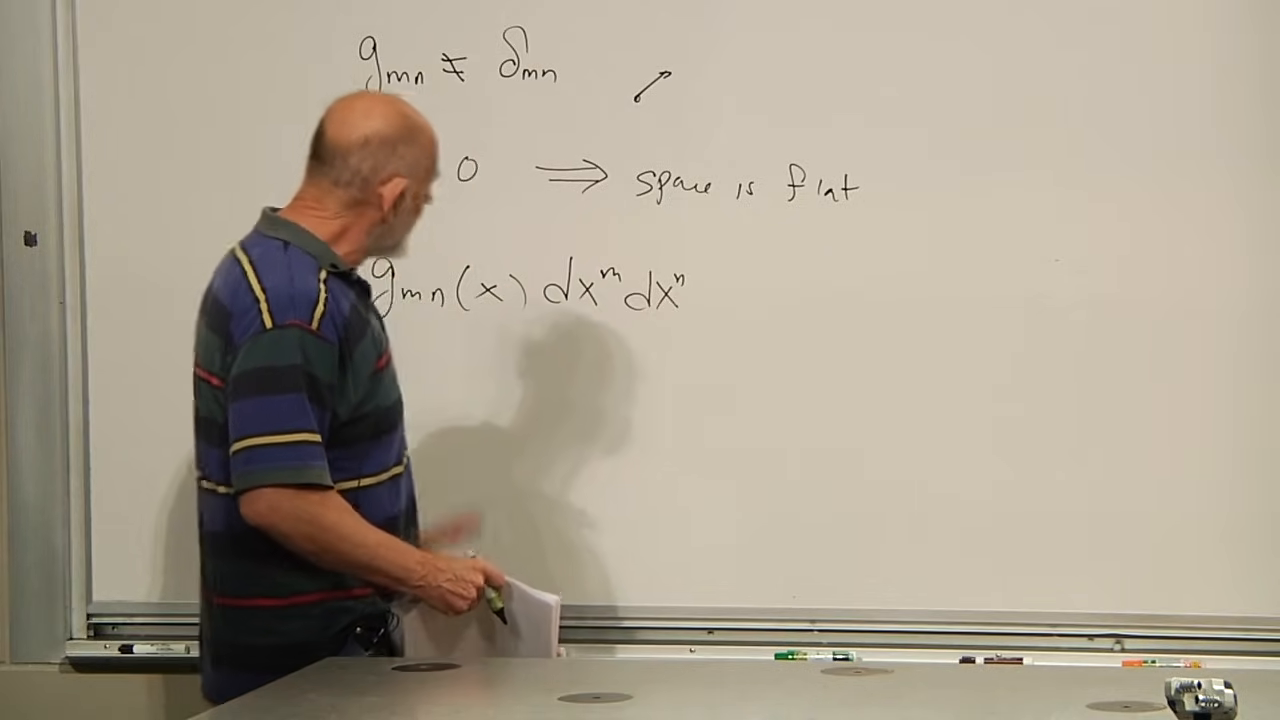
\includegraphics[width=\linewidth]{lecture_03_figure_02.png}
\caption{用依赖于位置的度规写出的不变线元。}
\lectureframe{00:19:00}
\end{figure}

度规是非退化的，因此有逆：
\begin{equation}
 g^{mn}g_{nr}=\delta^m{}_r.
\label{eq:l3-inverse-metric}
\end{equation}
混合的克罗内克张量\(\delta^m{}_r\)是恒等映射。在通常的黎曼几何中，度规还是正定的，
\begin{equation}
 g_{mn}u^m u^n>0
\qquad\text{for every nonzero }u^m.
\label{eq:l3-positive}
\end{equation}
洛伦兹时空稍后将放宽这一正定性，同时保留非退化性。

\begin{figure}[H]
\centering
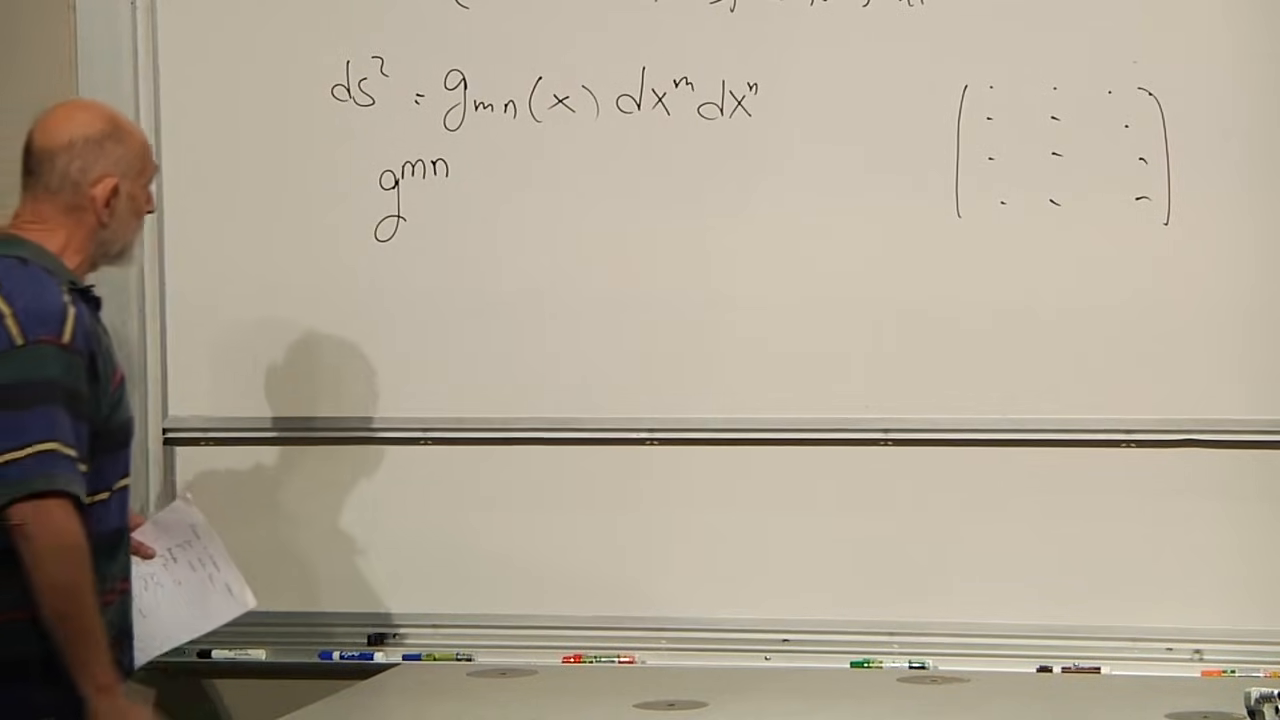
\includegraphics[width=\linewidth]{lecture_03_figure_03.png}
\caption{黑板上的逆度规与恒等张量。}
\lectureframe{00:20:40}
\end{figure}

度规将矢量与余矢量等同起来：
\begin{equation}
 V_m=g_{mn}V^n,
 \qquad
 V^m=g^{mn}V_n.
\label{eq:l3-raise-lower}
\end{equation}
因此，移动指标是由度规执行的一种操作，而不是排版上的改变。

\begin{figure}[H]
\centering
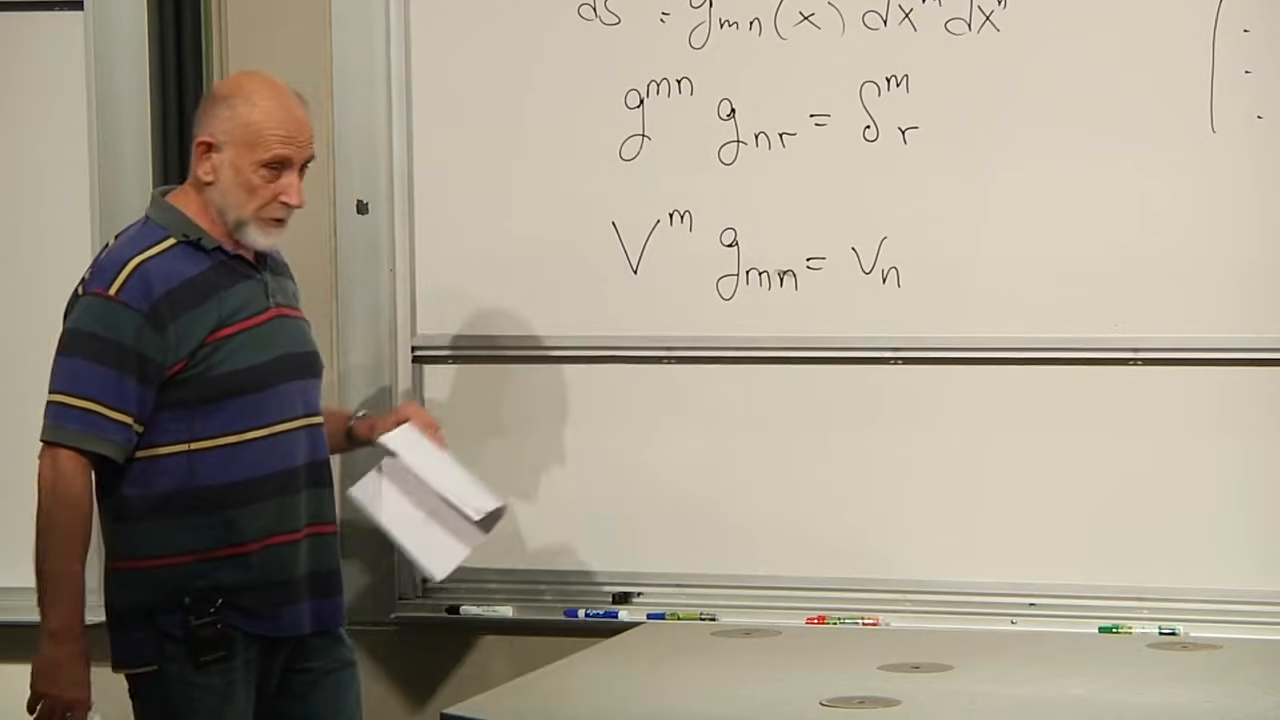
\includegraphics[width=\linewidth]{lecture_03_figure_04.png}
\caption{用度规及其逆来升降矢量指标。}
\lectureframe{00:24:40}
\end{figure}

如果在某个区域内\(g_{mn}\)的所有分量都是常数，那么一个常系数线性坐标变换可以在那里把度规对角化并归一化。此时几何就是平坦的。因此，有趣的信息必定与度规如何随位置变化有关。

\section{法坐标：一阶以内平坦}

选取一点\(P\)。法坐标定理说，可以构造以\(P\)为中心的坐标，使得
\begin{align}
 g_{mn}(P)&=\delta_{mn}, \label{eq:l3-normal-metric}\\
 \partial_r g_{mn}(P)&=0. \label{eq:l3-normal-first}
\end{align}
讲义称这些为高斯法坐标。从几何上看，就是过\(P\)画坐标轴，并让它们的坐标线在几何允许的范围内尽可能直地延伸。直线性的精确概念将成为测地运动。

\begin{figure}[H]
\centering
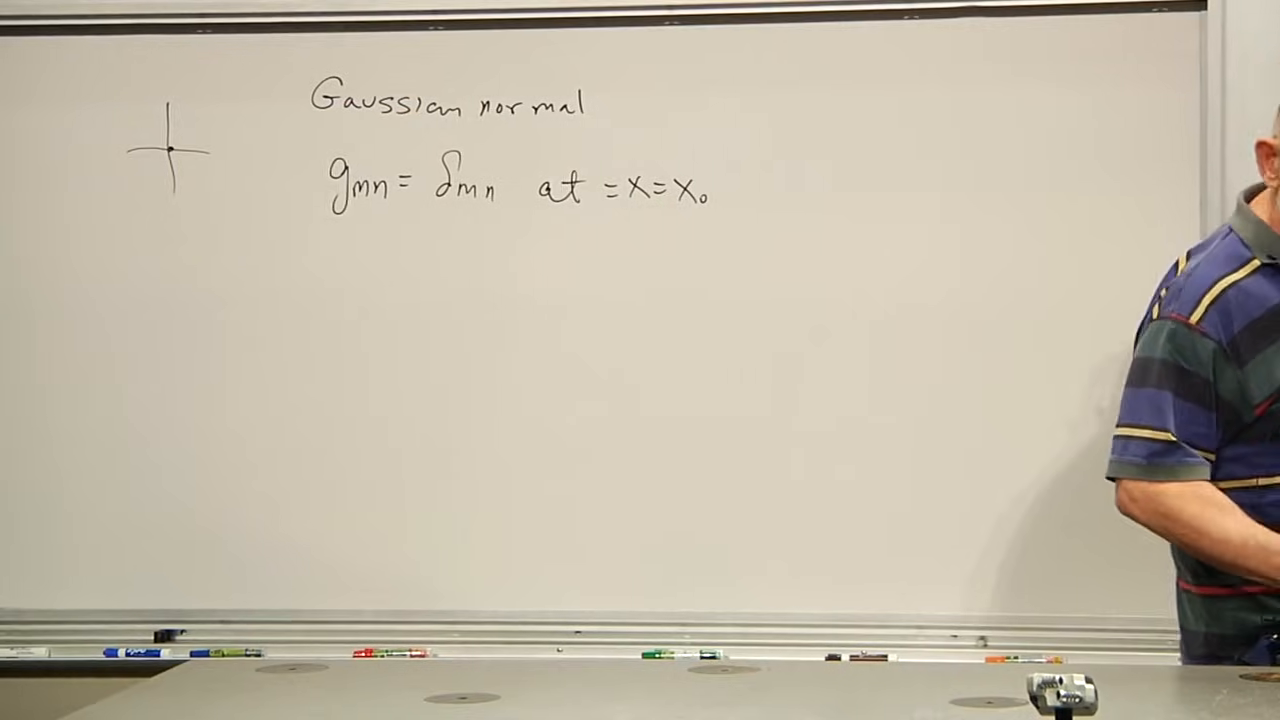
\includegraphics[width=\linewidth]{lecture_03_figure_05.png}
\caption{选取法坐标，使得度规在所选点处为欧几里得度规。}
\lectureframe{00:28:50}
\end{figure}

这样的标架并不唯一。在\(P\)处的一个正交旋转保持\(g_{mn}(P)=\delta_{mn}\)不变。重要的不是坐标轴的方向，而是存在一个标架，使得\eqref{eq:l3-normal-metric}和\eqref{eq:l3-normal-first}同时成立。

\begin{classroomqa}
\audiencequestion{这些条件只在所选点处成立，还是在一个邻域内处处成立？}
\lecturerresponse{它们在所选点\(P\)处成立。人们可以在任意点处建立法标架，但一般不能在一个弯曲区域上使用单一坐标系并处处保持度规为欧几里得度规且所有一阶导数都为零。把同一坐标从\(P\)向外延伸，就会暴露出度规的更高阶导数。
\lecturetimestamp{00:29:53}}
\end{classroomqa}

在\(P\)处，二阶导数一般是不可避免的：
\begin{equation}
 \partial_r\partial_s g_{mn}(P)\neq 0
 \qquad\text{in general}.
\label{eq:l3-normal-second}
\end{equation}
因此，度规在一个点处的零阶或一阶并不携带不变曲率信息；坐标自由度可以将其移除。第一个可能的不变信息出现在二阶。

\begin{figure}[H]
\centering
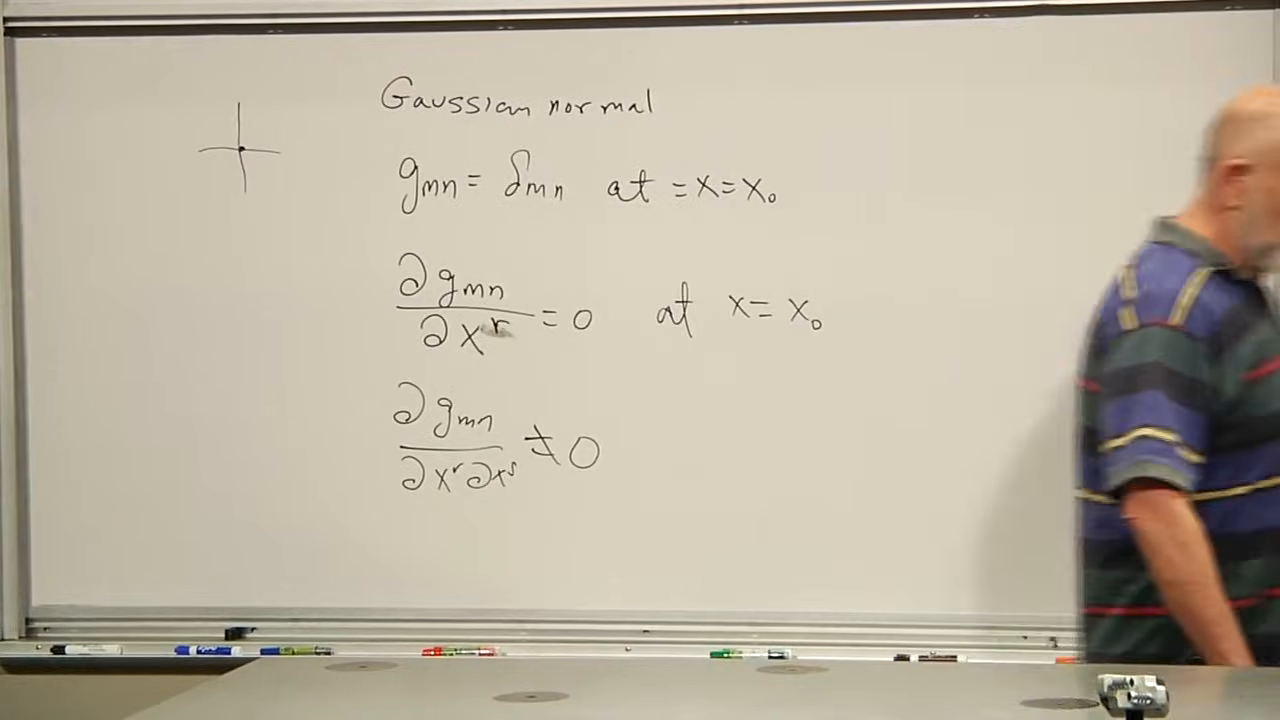
\includegraphics[width=\linewidth]{lecture_03_figure_06.png}
\caption{法坐标条件：度规为欧几里得度规，其一阶导数为零，而二阶导数不必为零。}
\lectureframe{00:30:50}
\end{figure}

\subsection{为什么坐标自由度是充分的}

取\(P\)为坐标\(x^m\)和\(y^m\)的公共原点。在用线性变换把原点处的度规安排好之后，考虑进一步坐标变换的二次部分：
\begin{equation}
 x^m
 =y^m+C^m{}_{nr}y^n y^r+O(y^3),
 \qquad C^m{}_{nr}=C^m{}_{rn}.
\label{eq:l3-quadratic-transform}
\end{equation}
在四维中，对称对\(nr\)有
\[
\frac{4(4+1)}{2}=10
\]
种独立选择。对于\(m\)的四个取值中的每一个，都有十个系数\(C^m{}_{nr}\)，从而给出四十个二次系数。

对称的度规在四维中同样有十个独立分量。每个分量有四个一阶导数，因此条件\(\partial_r g_{mn}(P)=0\)包含四十个方程。数量上的匹配表明，二次坐标自由度的大小恰好足以施加这些一阶导数条件。正规坐标定理提供了存在性陈述；仅靠计数只是一种有用的结构性检验，而不是对任意非线性系统可解性的完整证明。

\begin{figure}[H]
\centering
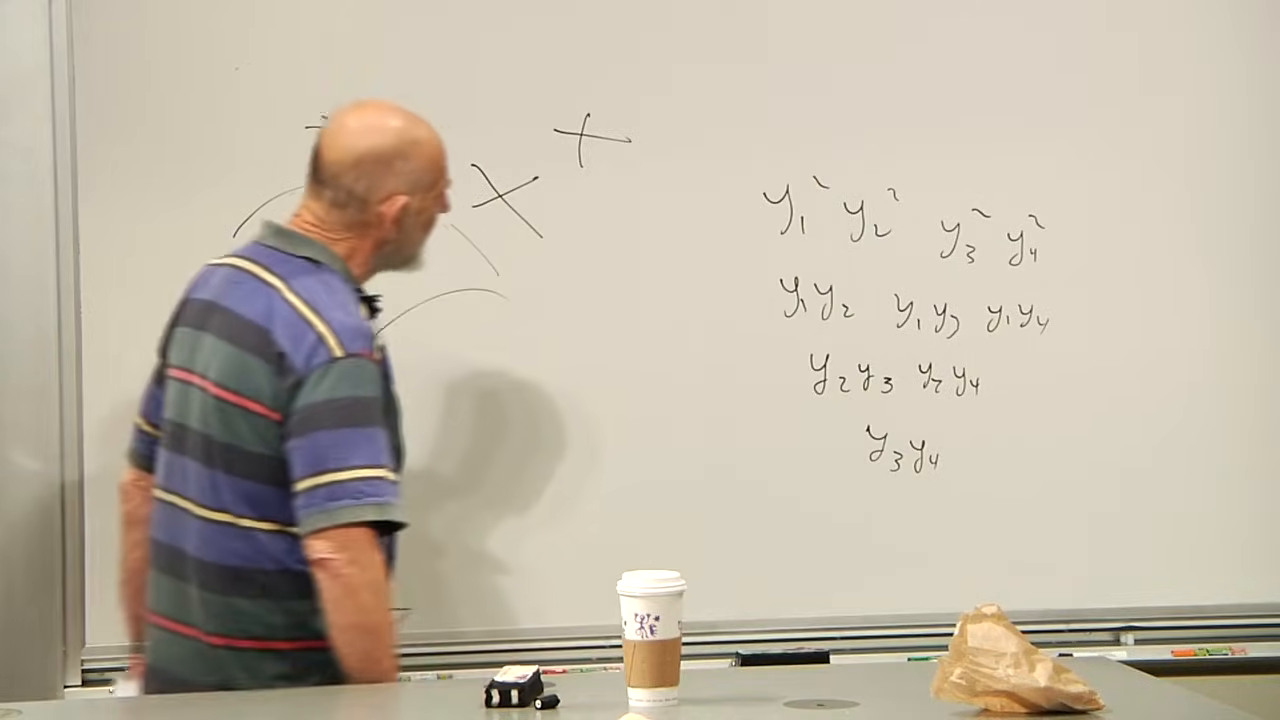
\includegraphics[width=\linewidth]{lecture_03_figure_07.png}
\caption{二次坐标变换与四维中十个独立的二次单项式。}
\lectureframe{00:33:50}
\end{figure}

\begin{classroomqa}
\audiencequestion{\(x^m=y^m+C^m{}_{nr}y^n y^r+\cdots\)是否是一种尝试性的坐标变换？}
\lecturerresponse{是的。系数\(C^m{}_{nr}\)的选取使得在新坐标下，度规的一阶导数在共同原点处为零。线性部分使雅可比行列式在该点附近保持可逆，而二次部分则调整度规的一阶导数。\lecturetimestamp{00:35:41}}
\end{classroomqa}

\begin{classroomqa}
\audiencequestion{这是否就是所谓光滑几何局部平坦的含义？}
\lecturerresponse{这是相关的一阶陈述。在足够小的尺度上，光滑曲面由其切平面近似，而正规坐标通过\(g_{mn}(P)=\delta_{mn}\)和\(\partial_r g_{mn}(P)=0\)表达了这一事实。在某个邻域上精确平坦则更强：它还要求曲率张量在该处为零。\lecturetimestamp{00:36:19}}
\end{classroomqa}

\begin{classroomqa}
\audiencequestion{四十个系数与四十个方程之间的相等真的能确保这些方程可解吗？}
\lecturerresponse{计数确定了所需的坐标自由度，而定理则保证了光滑非退化度规的局部构造。讲座提议将二维情形作为练习直接检验。该论证并不依赖于四维；在\(d\)维中，同样的对称性与坐标自由度相互契合。\lecturetimestamp{00:36:45}}
\end{classroomqa}

\begin{classroomqa}
\audiencequestion{为什么展开式中没有常数项，哪一项是一阶项？}
\lecturerresponse{\(y^m\)项是一阶项。常数项被省略，是因为两个坐标原点被特意选为表示同一点，因此\(y=0\)蕴含\(x=0\)。这一选择不损失任何一般性。\lecturetimestamp{00:38:52}}
\end{classroomqa}

\section{为何逐分量微分不成立}

现在考虑一个协变矢量场\(V_m(x)\)。在平坦空间的直线笛卡尔坐标中，几何上恒定的矢量具有恒定的分量。因此人们可能试图将其导数定义为\(\partial_rV_m\)。一旦坐标网格弯曲，困难就出现了。

\begin{figure}[H]
\centering
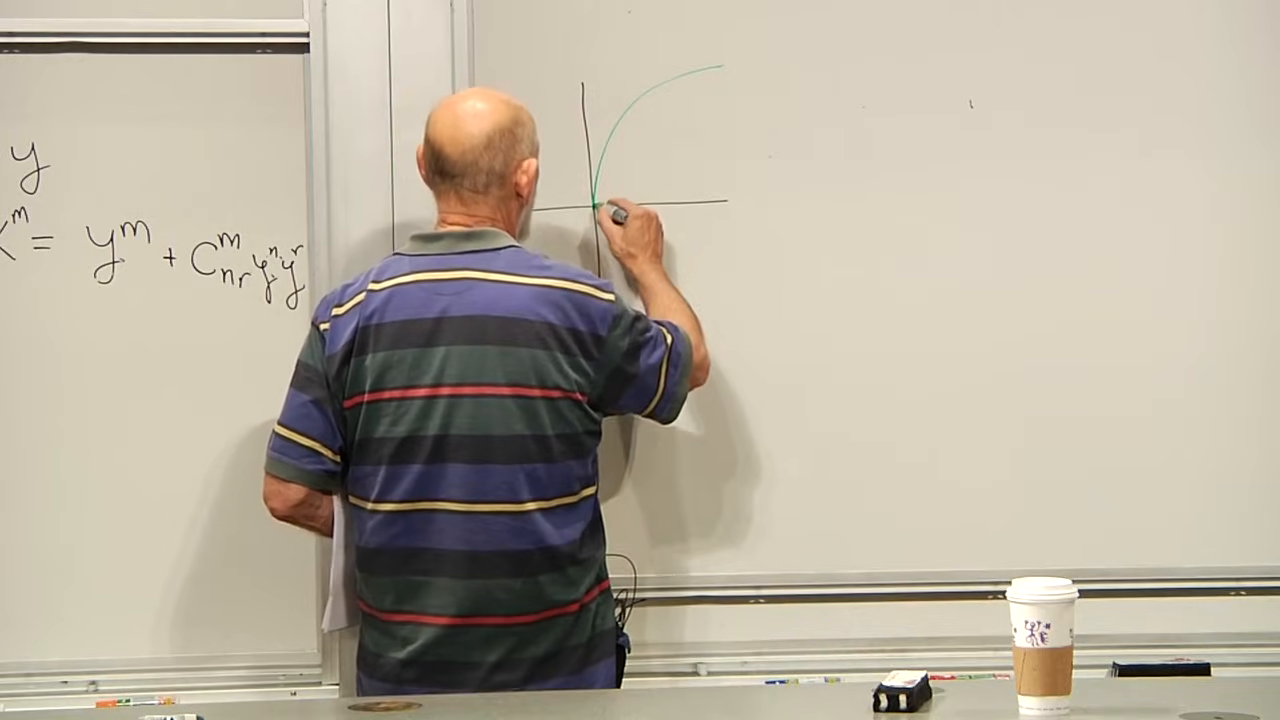
\includegraphics[width=\linewidth]{lecture_03_figure_08.png}
\caption{叠加在局部直线参考系上的曲线坐标网格。}
\lectureframe{00:40:10}
\end{figure}

将同一个几何矢量置于相邻点上。相对于固定的笛卡尔参考系，其分量不变。然而相对于曲线基，基矢量本身在移动时发生转动，因此即使矢量不变，其分量列表也会改变。

\begin{figure}[H]
\centering
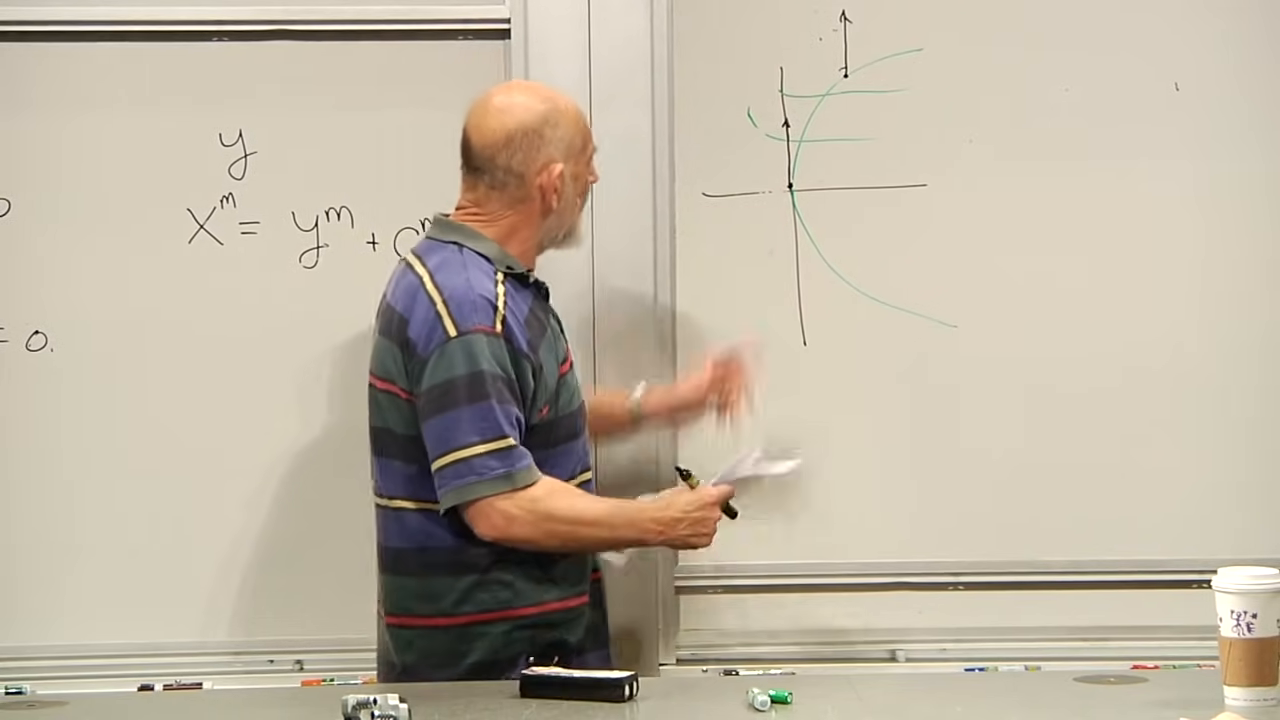
\includegraphics[width=\linewidth]{lecture_03_figure_09.png}
\caption{同一个矢量在相邻点处获得不同的分量，因为局部坐标基发生了旋转。}
\lectureframe{00:42:30}
\end{figure}

因此，朴素条件
\begin{equation}
 \partial_rV_m=0
\label{eq:l3-naive-derivative}
\end{equation}
可能在一个坐标系中成立而在另一个坐标系中不成立。如果\(\partial_rV_m\)是一个二阶张量，那将是不可能的：在一个参考系中为零将意味着在每个参考系中为零。因此，矢量分量的普通偏导数不是张量分量。

\begin{figure}[H]
\centering
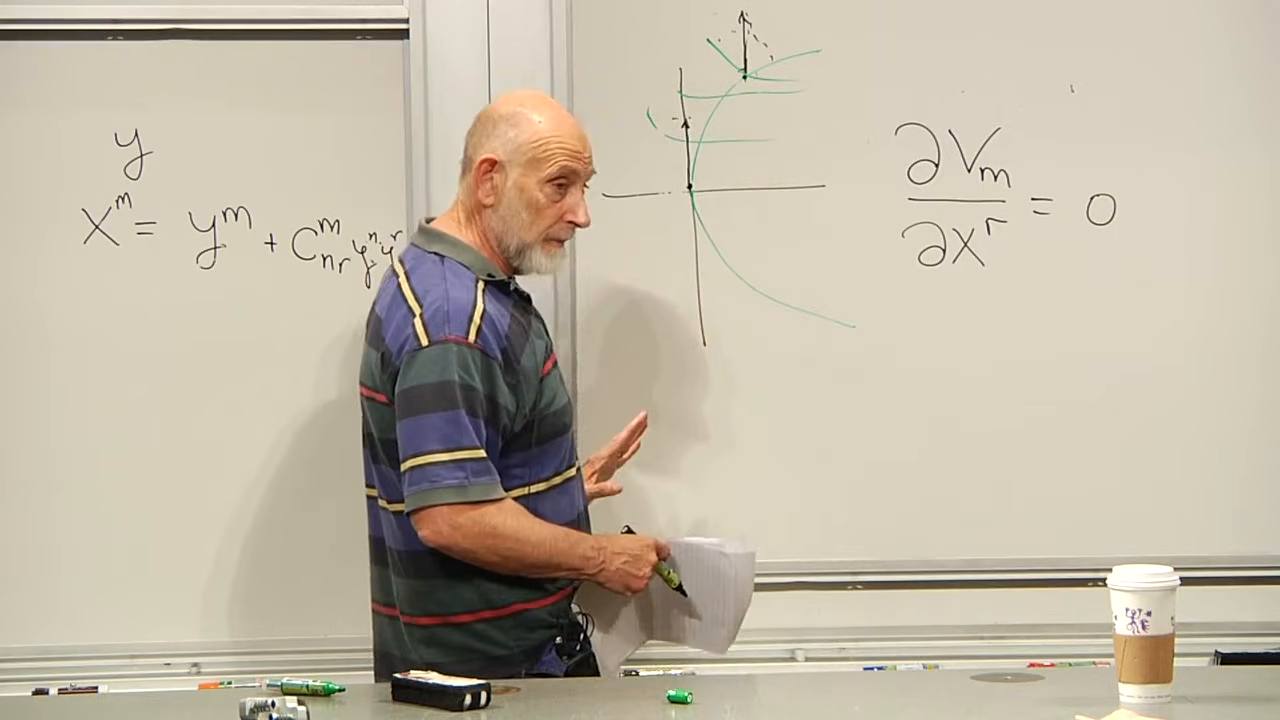
\includegraphics[width=\linewidth]{lecture_03_figure_10.png}
\caption{刻意朴素的零导数条件与变化的曲线基并列。}
\lectureframe{00:44:00}
\end{figure}

我们需要一种导数，它能消除由基引起的表观变化，同时保留矢量场的真实变化。

\section{定义协变导数}

在\(P\)处的微分只比较\(P\)的任意小邻域内的值。因此我们可以从以该点为中心的正规坐标出发。取相邻点处的一个矢量，将其尾部平移回\(P\)，并在平移过程中保持其正规坐标分量不变。将平移后的矢量与已经在\(P\)处的矢量进行比较，再除以间隔，就得到该局部直线参考系中的普通导数。

\begin{figure}[H]
\centering
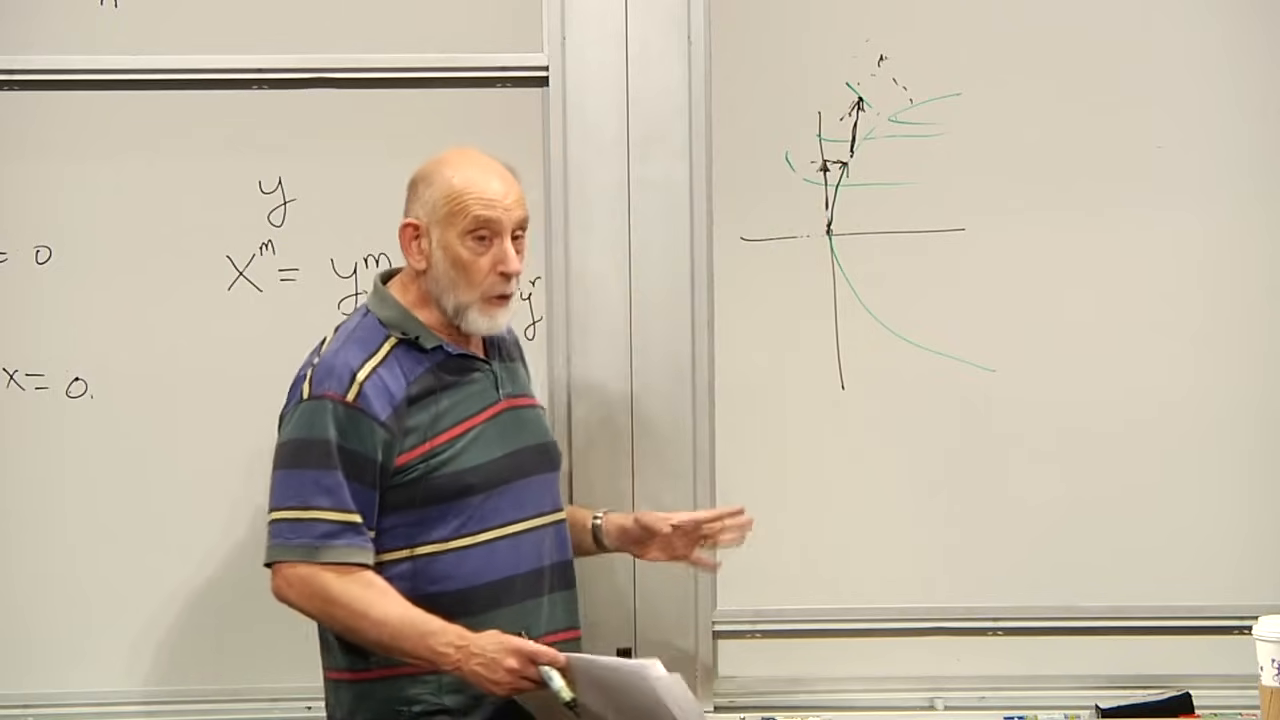
\includegraphics[width=\linewidth]{lecture_03_figure_11.png}
\caption{局部比较：在取差之前，先在正规坐标中平移相邻矢量。}
\lectureframe{00:46:50}
\end{figure}

现在把那个几何定义的导数用任意坐标表示出来。这里有两项贡献：分量\(V_m\)可能改变，坐标基也可能改变。指标结构决定了修正项的形式：
\begin{equation}
 \nabla_rV_m
 =\partial_rV_m-\Gamma^t{}_{rm}V_t.
\label{eq:l3-covector-derivative}
\end{equation}
量\(\Gamma^t{}_{rm}\)称为联络系数，也叫克里斯托费尔符号。负号对于下指标矢量是恰当的。在正规坐标的中心\(P\)处，
\begin{equation}
 \Gamma^t{}_{rm}(P)=0,
\qquad
 \nabla_rV_m(P)=\partial_rV_m(P).
\label{eq:l3-gamma-normal-zero}
\end{equation}

\begin{figure}[H]
\centering
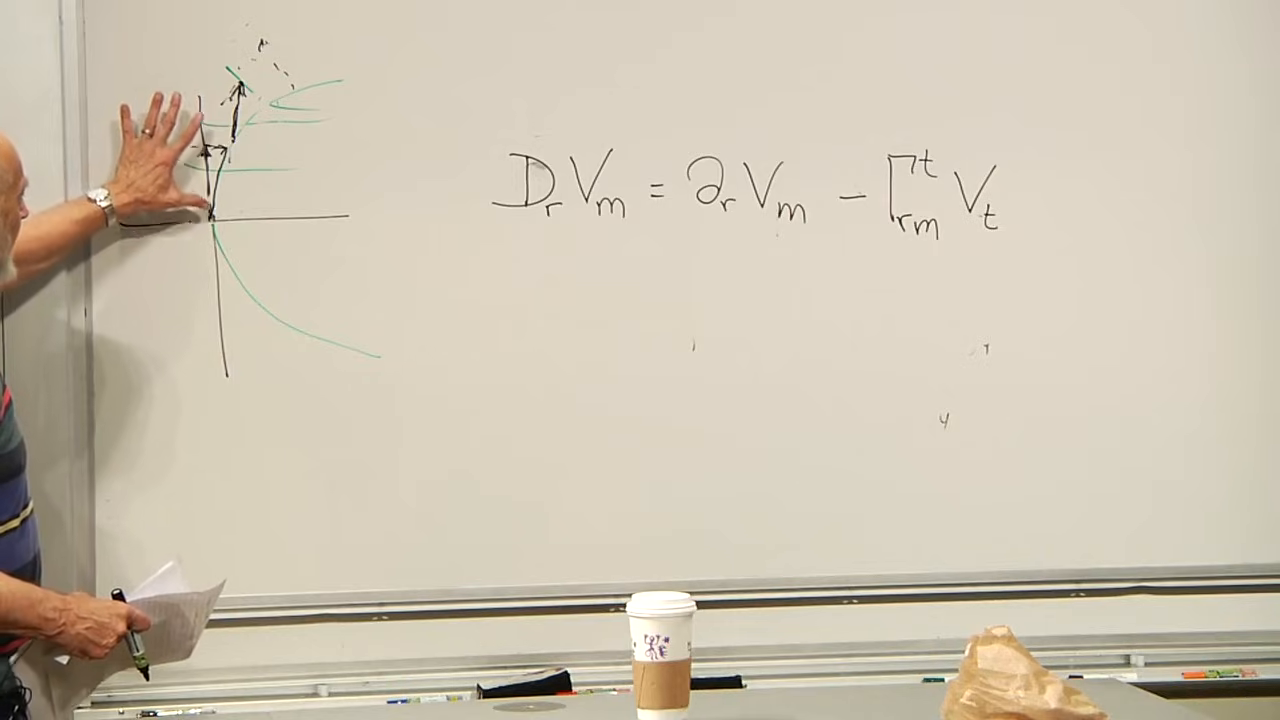
\includegraphics[width=\linewidth]{lecture_03_figure_12.png}
\caption{协变导数作用于余向量：普通的分量变化减去由运动基矢引起的变化。}
\lectureframe{00:49:50}
\end{figure}

\begin{classroomqa}
\audiencequestion{在任意坐标下
\(\nabla_rV_m=\partial_rV_m-\Gamma^t{}_{rm}V_t\)是否成立，而在正规坐标下它又变成什么？}
\lecturerresponse{完整的公式在任意坐标下都成立。在正规坐标中所选的点处，度规的一阶导数因而克里斯托费尔符号都为零，只剩下
\(\partial_rV_m\)。离开该点后，即使同一套正规坐标图一般也具有非零的联络系数。
\lecturetimestamp{00:50:22}}
\end{classroomqa}

协变导数之所以如此命名，是因为整个对象\(\nabla_rV_m\)作为张量协变地变换；这个名字并不仅仅是对下导数指标的评论。克里斯托费尔项恰恰修补了偏导数非张量的变换。

\begin{figure}[H]
\centering
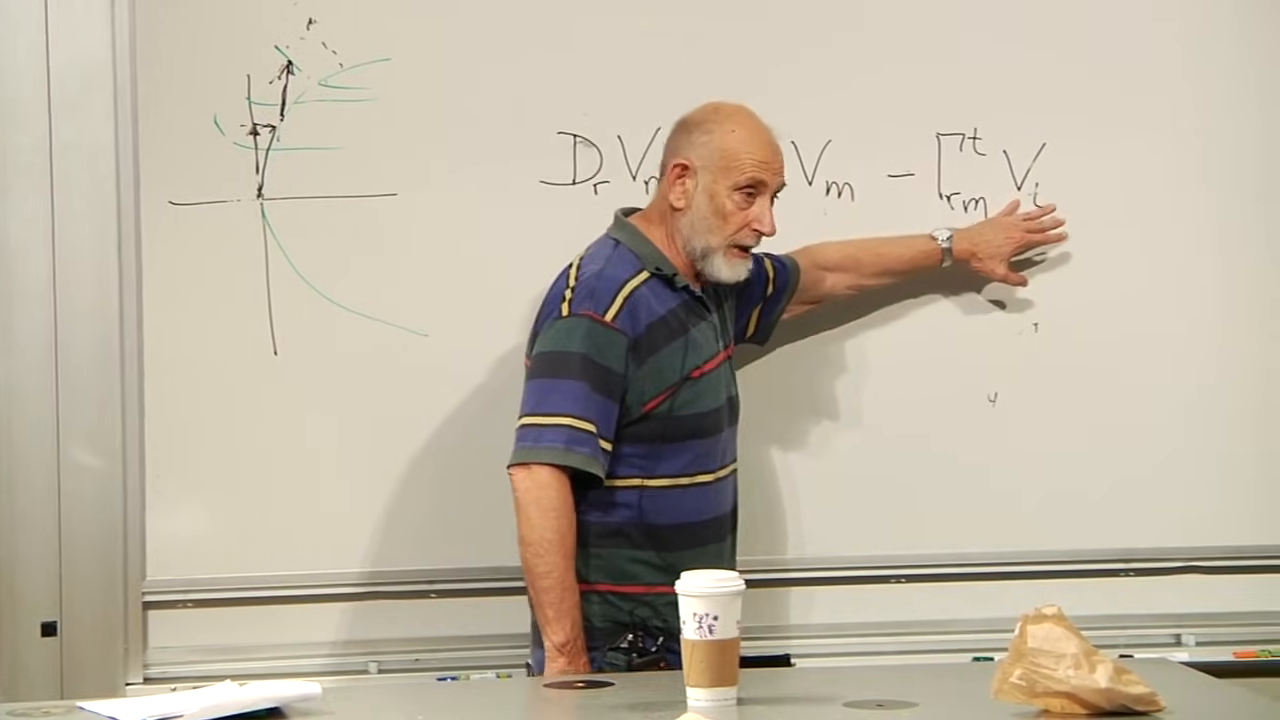
\includegraphics[width=\linewidth]{lecture_03_figure_13.png}
\caption{完整的余矢量导数及其联络修正。}
\lectureframe{00:51:30}
\end{figure}

\begin{classroomqa}
\audiencequestion{这与流体流动中使用的对流导数有关吗？}
\lecturerresponse{讲座谨慎地回答说，二者有联系：流体力学也区分由流动携带的变化与在固定坐标点看到的变化，而在弯曲坐标或弯曲空间上的流体方程中会出现协变导数。这两个算子按定义并不相同，但都对朴素的导数作了修正，以顾及随描述而运动的结构。
\lecturetimestamp{00:52:31}}
\end{classroomqa}

对于这里所用的无挠联络，
\begin{equation}
 \Gamma^t{}_{rm}=\Gamma^t{}_{mr}.
\label{eq:l3-torsion-free}
\end{equation}
更一般的几何可以具有挠率，不必满足这一对称性。当前的联络正是与广义相对论的标准度规表述相关的那个联络。

\begin{figure}[H]
\centering
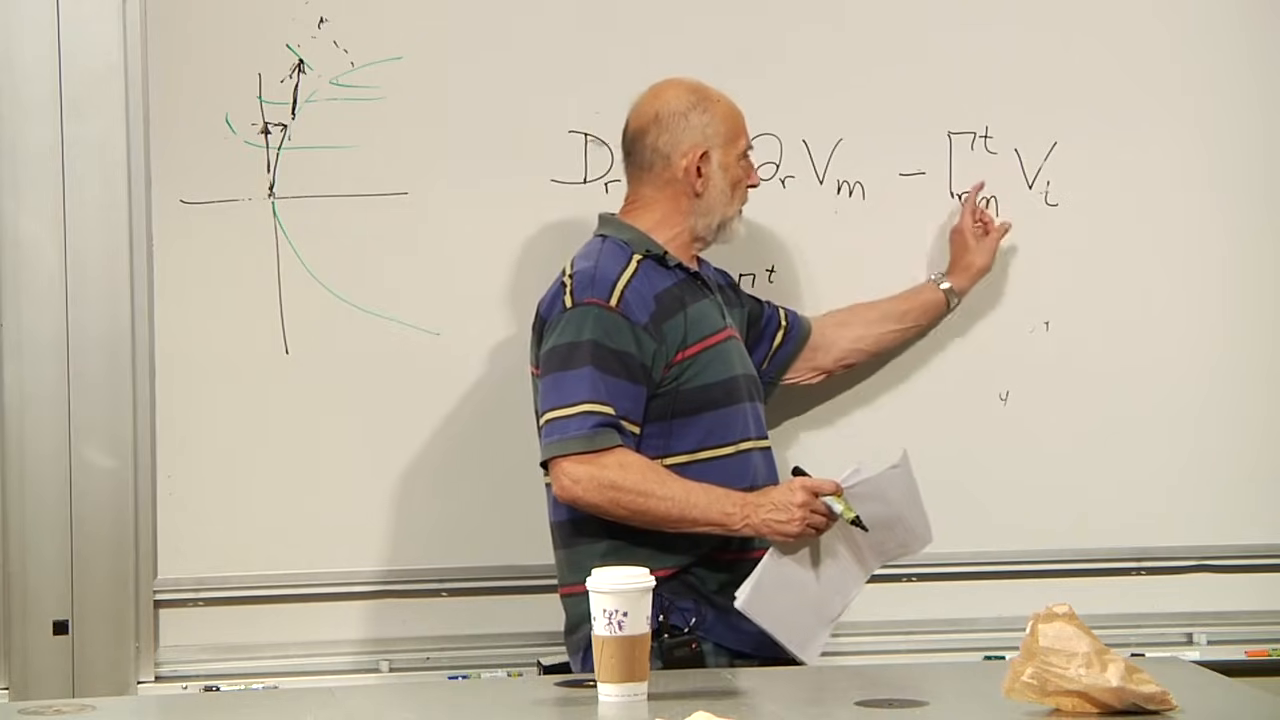
\includegraphics[width=\linewidth]{lecture_03_figure_14.png}
\caption{克里斯托费尔符号被认定为无挠几何的对称联络系数。}
\lectureframe{00:54:30}
\end{figure}

有一个有用的物理类比。正规坐标在一个事件处扮演自由下落参考系的角色：在那里可以使坐标修正消失。任意曲线坐标则类似于加速电梯，其中因为参考系本身在变化而出现表观力。这个类比是局部的，而曲率将衡量为什么单一的自由下落参考系无法在一个延展的区域内消除引力。

\subsection{每个张量指标对应一项修正}

对于协变二阶张量\(T_{mn}\)，每个下指标都得到自己的联络修正：
\begin{equation}
 \nabla_sT_{mn}
 =\partial_sT_{mn}
 -\Gamma^t{}_{sm}T_{tn}
 -\Gamma^t{}_{sn}T_{mt}.
\label{eq:l3-rank-two-derivative}
\end{equation}
要记住这条规则，可以在对另一个指标求导时把一个指标固定为旁观者，然后对第二个指标重复这一做法。逆变指标则得到符号相反的相应项。

\begin{figure}[H]
\centering
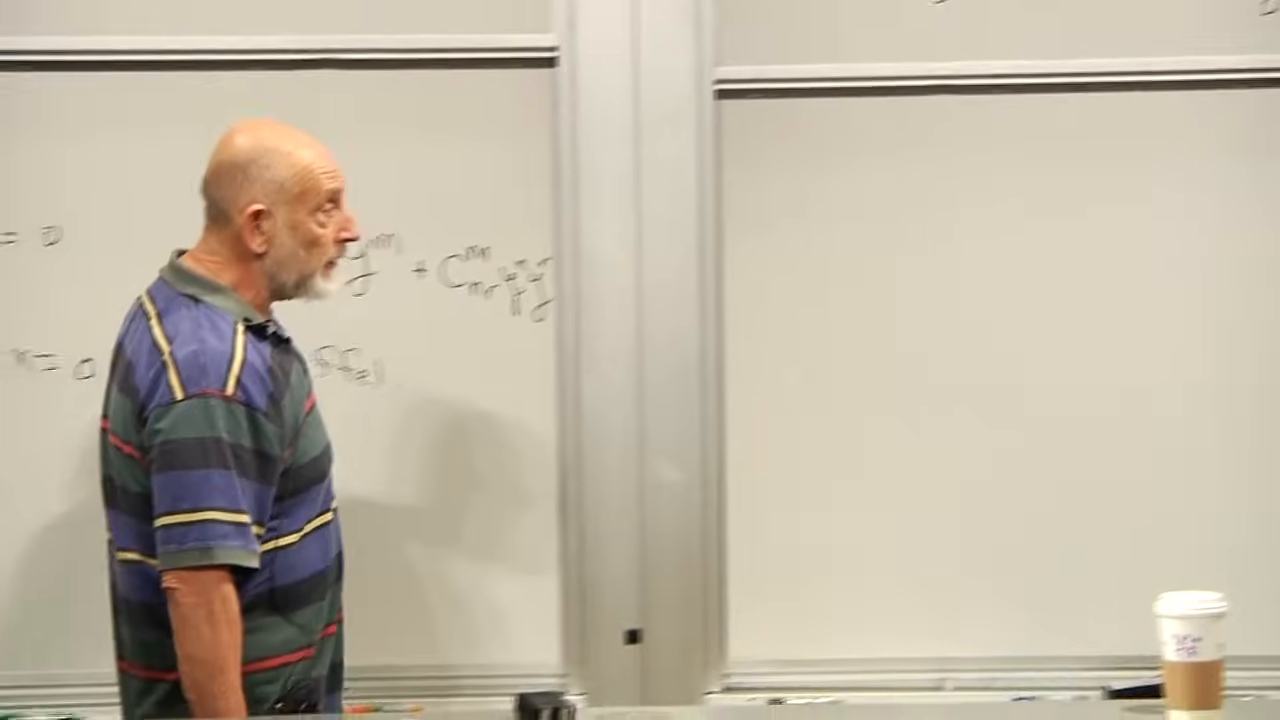
\includegraphics[width=\linewidth]{lecture_03_figure_15.png}
\caption{二阶协变张量的协变导数，每个下指标对应一项克里斯托费尔修正。}
\lectureframe{01:01:50}
\end{figure}

\begin{classroomqa}
\audiencequestion{符号\(\partial_r\)本身是否只指正规坐标，而张量公式是否只限于那个参考系？}
\lecturerresponse{不是。记号
\(\partial_r=\partial/\partial x^r\)在任何坐标系中都有意义，而完整的协变导数公式是为任意坐标写出的。只有在正规参考系中所选的点处，克里斯托费尔修正才消失。\lecturetimestamp{00:57:22}}
\end{classroomqa}

\begin{classroomqa}
\audiencequestion{当协变导数在正规坐标下化为偏导数时，这种化简是否只在所选的点处成立？克里斯托费尔符号是张量吗？}
\lecturerresponse{是的，这种化简是逐点的。克里斯托费尔符号不是张量：它们可以在正规坐标下于\(P\)处为零，而在另一坐标系中的同一点处非零。它们的非张量变换恰恰使得\eqref{eq:l3-covector-derivative}中的组合能够作为张量变换。
\lecturetimestamp{00:58:13}}
\end{classroomqa}

\begin{classroomqa}
\audiencequestion{协变导数实际上将用于什么？}
\lecturerresponse{用于场方程。引力场逐点变化，因此其方程必须包含导数。同时，方程在每个坐标系中应具有相同的内容。协变微分将张量变为张量，因此允许其真理性不依赖于特定参考系的微分方程。\lecturetimestamp{01:02:35}}
\end{classroomqa}

\begin{classroomqa}
\audiencequestion{协变导数能否乘以坐标微分来描述相邻点之间的变化？}
\lecturerresponse{可以。沿无穷小位移\(dx^s\)，协变变化为\(dx^s\nabla_sT\)。偏导数项度量分量的变化，而联络项则说明坐标基的变化。即使在极坐标下的平坦空间也需要这一区分。\lecturetimestamp{01:03:22}}
\end{classroomqa}

\section{度规相容性决定联络}

将二阶规则应用于度规。在正规坐标中的\(P\)处，\(\partial_sg_{mn}=0\)且\(\Gamma^t{}_{sm}=0\)，因此\(\nabla_sg_{mn}=0\)。由于协变导数是张量，这一逐点结果在每个坐标系中都成立：
\begin{equation}
 \nabla_sg_{mn}=0.
\label{eq:l3-metric-compatibility}
\end{equation}
这就是度规相容性。它表明平行移动保持度规，因而保持长度和角度。

\begin{figure}[H]
\centering
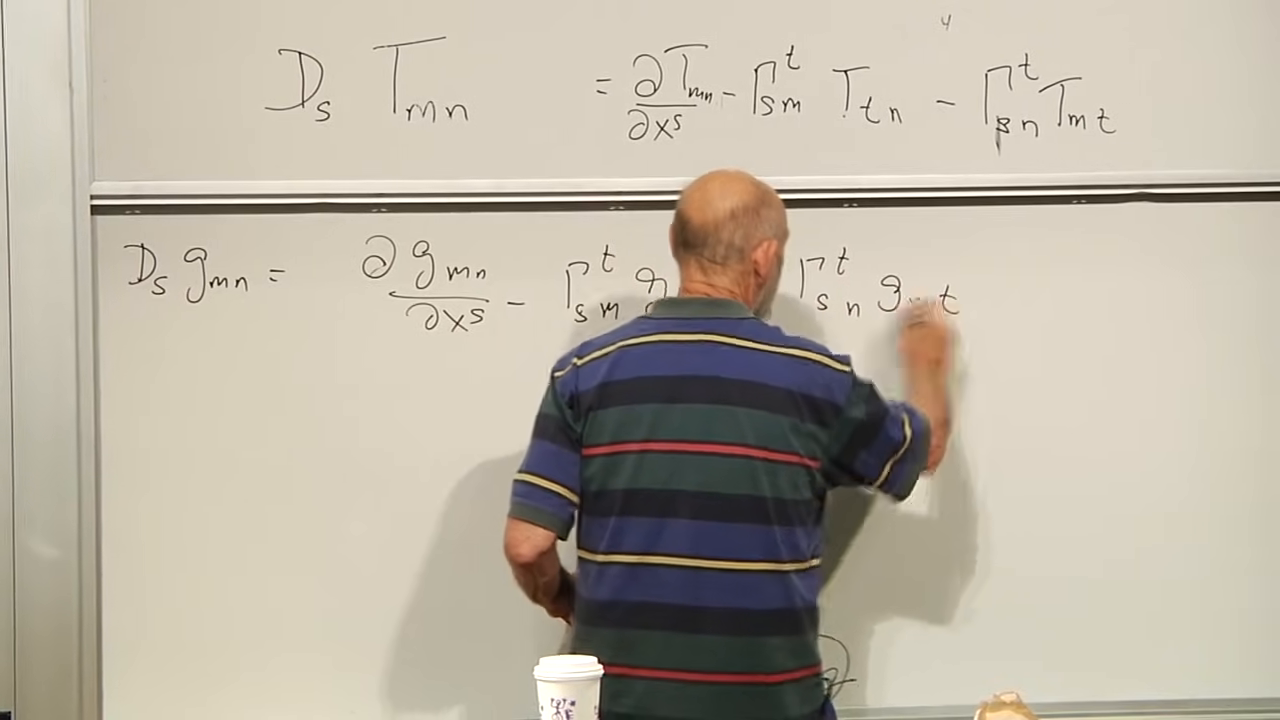
\includegraphics[width=\linewidth]{lecture_03_figure_16.png}
\caption{度规相容性方程开启了从度规推导联络的过程。}
\lectureframe{01:06:20}
\end{figure}

展开\eqref{eq:l3-metric-compatibility}得到
\begin{equation}
 0
 =\partial_sg_{mn}
 -\Gamma^t{}_{sm}g_{tn}
 -\Gamma^t{}_{sn}g_{mt}.
\label{eq:l3-compat-expanded}
\end{equation}
再写出两份，将导数指标与度规指标循环置换：
\begin{align}
 0
 &=\partial_mg_{sn}
 -\Gamma^t{}_{ms}g_{tn}
 -\Gamma^t{}_{mn}g_{st},
\label{eq:l3-compat-m}\\
 0
 &=\partial_ng_{sm}
 -\Gamma^t{}_{ns}g_{tm}
 -\Gamma^t{}_{nm}g_{st}.
\label{eq:l3-compat-n}
\end{align}

\begin{figure}[H]
\centering
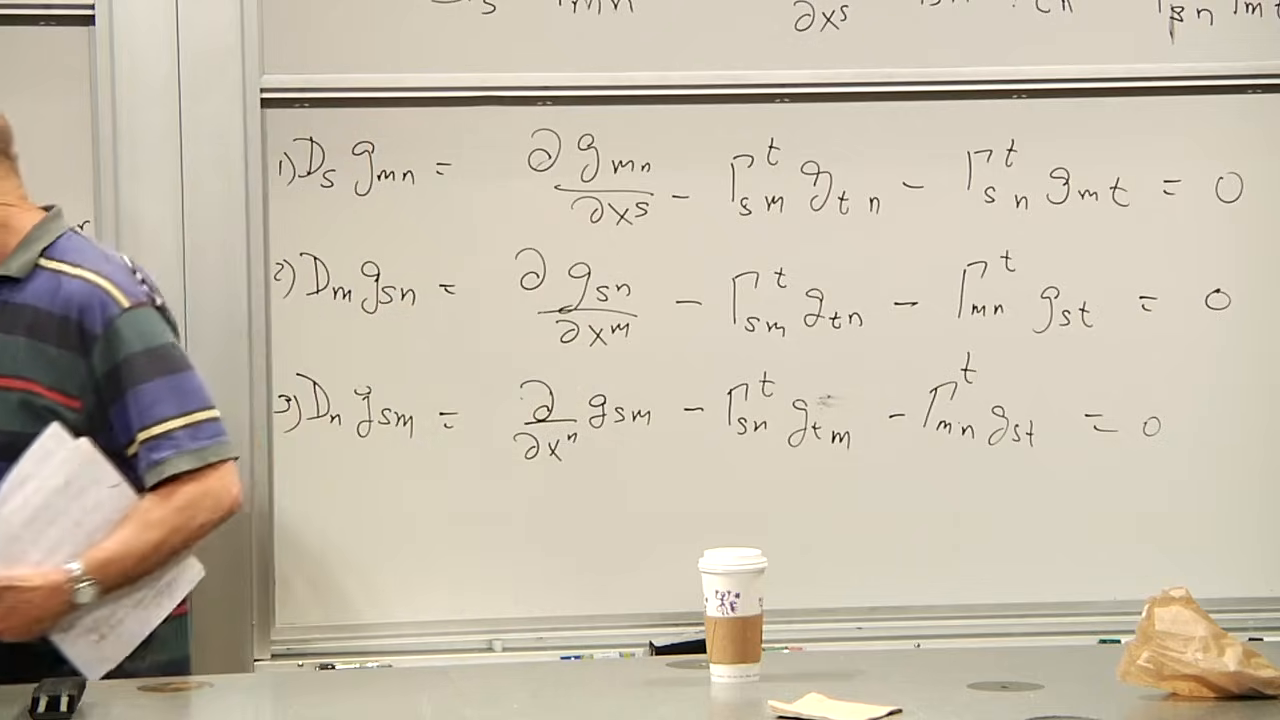
\includegraphics[width=\linewidth]{lecture_03_figure_17.png}
\caption{三个指标置换后的度规相容性方程。}
\lectureframe{01:10:20}
\end{figure}

将\eqref{eq:l3-compat-m}与\eqref{eq:l3-compat-n}相加，
再减去\eqref{eq:l3-compat-expanded}。利用无挠对称性\eqref{eq:l3-torsion-free}，不需要的联络项相消：
\begin{equation}
 \partial_mg_{sn}+\partial_ng_{sm}-\partial_sg_{mn}
 =2\Gamma^t{}_{mn}g_{st}.
\label{eq:l3-isolate-gamma-lowered}
\end{equation}

\begin{figure}[H]
\centering
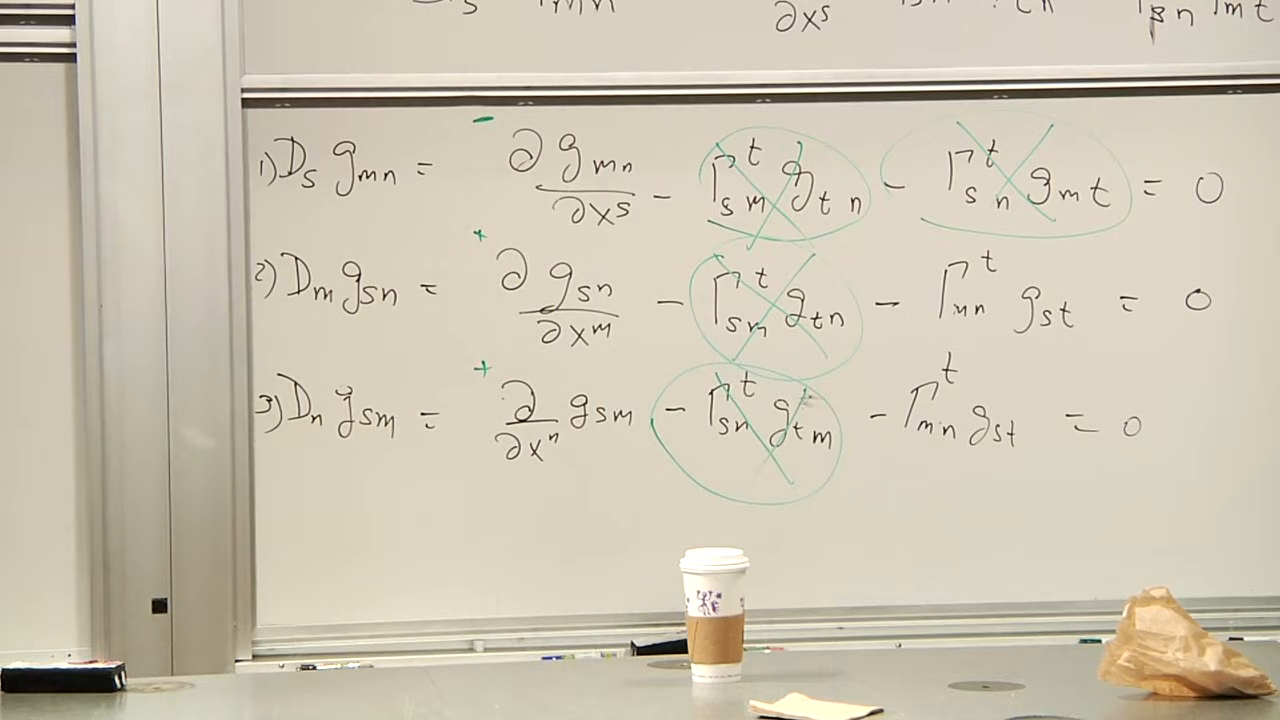
\includegraphics[width=\linewidth]{lecture_03_figure_18.png}
\caption{将两个相容性方程相加并减去第三个，消去了不需要的克里斯托费尔项。}
\lectureframe{01:12:10}
\end{figure}

乘以\(g^{rs}\)可分离出联络：
\begin{equation}
 \boxed{
 \Gamma^r{}_{mn}
 =\frac12 g^{rs}
 \left(
 \partial_mg_{sn}
 +\partial_ng_{sm}
 -\partial_sg_{mn}
 \right)}
\label{eq:l3-christoffel}
\end{equation}
因此列维-奇维塔联络由度规及其一阶导数构成。这就是所承诺的克里斯托费尔符号在正规坐标中心处为零的原因。

\begin{figure}[H]
\centering
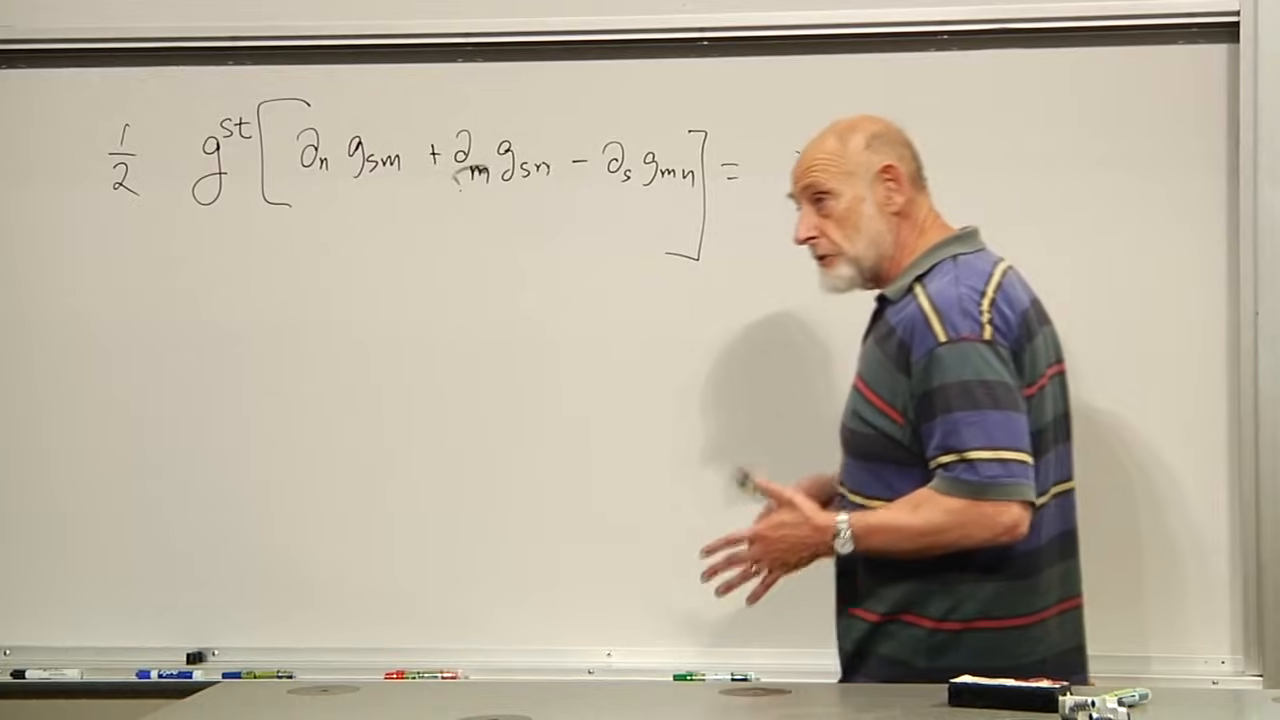
\includegraphics[width=\linewidth]{lecture_03_figure_19.png}
\caption{逆度规从降指标的联络方程中分离出克里斯托费尔符号。}
\lectureframe{01:16:10}
\end{figure}

\begin{classroomqa}
\audiencequestion{为什么三个度规相容性方程都被设为零？}
\lecturerresponse{在正规坐标中所选的点处，度规的普通导数消失，克里斯托费尔符号也消失。因此度规的协变导数在该处为零。要在任何其他点确立这一陈述，就在该点建立正规标架并重复。由于\(\nabla_sg_{mn}\)是张量，其为零与坐标无关。\lecturetimestamp{01:14:27}}
\end{classroomqa}

\begin{classroomqa}
\audiencequestion{度规和克里斯托费尔数组的维数是多少，为什么四维中有四十个独立的克里斯托费尔分量？}
\lecturerresponse{在\(d\)维中，\(g_{mn}\)是一个对称的\(d\times d\)矩阵。联络有三个指标。对每个固定的上指标\(r\)，对称的下指标对\(mn\)有\(d(d+1)/2\)种选择。因此无挠联络有\(d^2(d+1)/2\)个独立分量，当\(d=4\)时为四十。\lecturetimestamp{01:16:18}}
\end{classroomqa}

\begin{figure}[H]
\centering
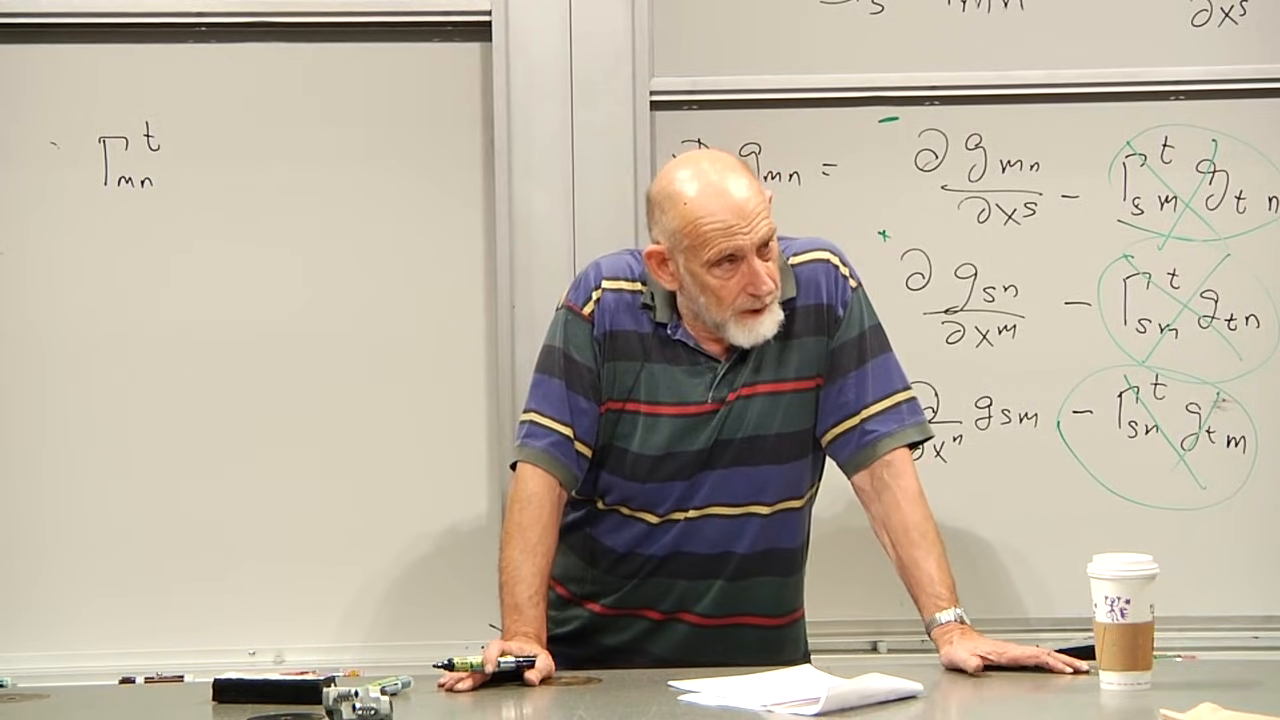
\includegraphics[width=\linewidth]{lecture_03_figure_20.png}
\caption{分量计数讨论时的板书：对称下指标对有十种选择，上指标有四种选择。}
\lectureframe{01:16:30}
\end{figure}

\begin{classroomqa}
\audiencequestion{\eqref{eq:l3-christoffel}中出现的是哪个度规？是否必须在每一点使用不同的正规坐标度规？}
\lecturerresponse{该公式使用度规在计算所选用的任何整体或局部坐标中的分量。正规坐标只是用于推导该规则的局部工具：在一点转到正规标架，在那里求导，将结果变换回来，然后丢弃辅助标架。一旦\eqref{eq:l3-christoffel}已知，就直接在感兴趣的任意坐标中求值。\lecturetimestamp{01:17:21}}
\end{classroomqa}

\begin{classroomqa}
\audiencequestion{无论是\(\nabla_sg_{mn}=0\)还是克里斯托费尔公式，是否都告诉我们空间是平坦的？}
\lecturerresponse{不是。度规相容性对每一个列维-奇维塔联络都成立，无论弯曲还是平坦。即使在用极坐标写出的平坦平面上，克里斯托费尔符号也可以非零。如果在一个图册的某个区域内所有\(\Gamma^r{}_{mn}\)都为零，那么该图册在那里就是笛卡儿坐标，该区域是平坦的；但仅凭它们非零并不能诊断曲率。仍然需要一个由\(\Gamma\)的导数与乘积构成的张量。\lecturetimestamp{01:19:27}}
\end{classroomqa}

\section{圆锥揭示联络所不能揭示的东西}

考虑一个圆滑的圆锥。在远离其尖端处，它可以用纸做的普通圆锥来近似。从一张平圆盘上切下一个楔形，再把露出的边缘粘在一起。剩下的纸没有任何拉伸；局部地看，除接缝和尖端外的每一点仍然是平坦的。缺失的楔形由亏角\(\Delta\)记录。

\begin{figure}[H]
\centering
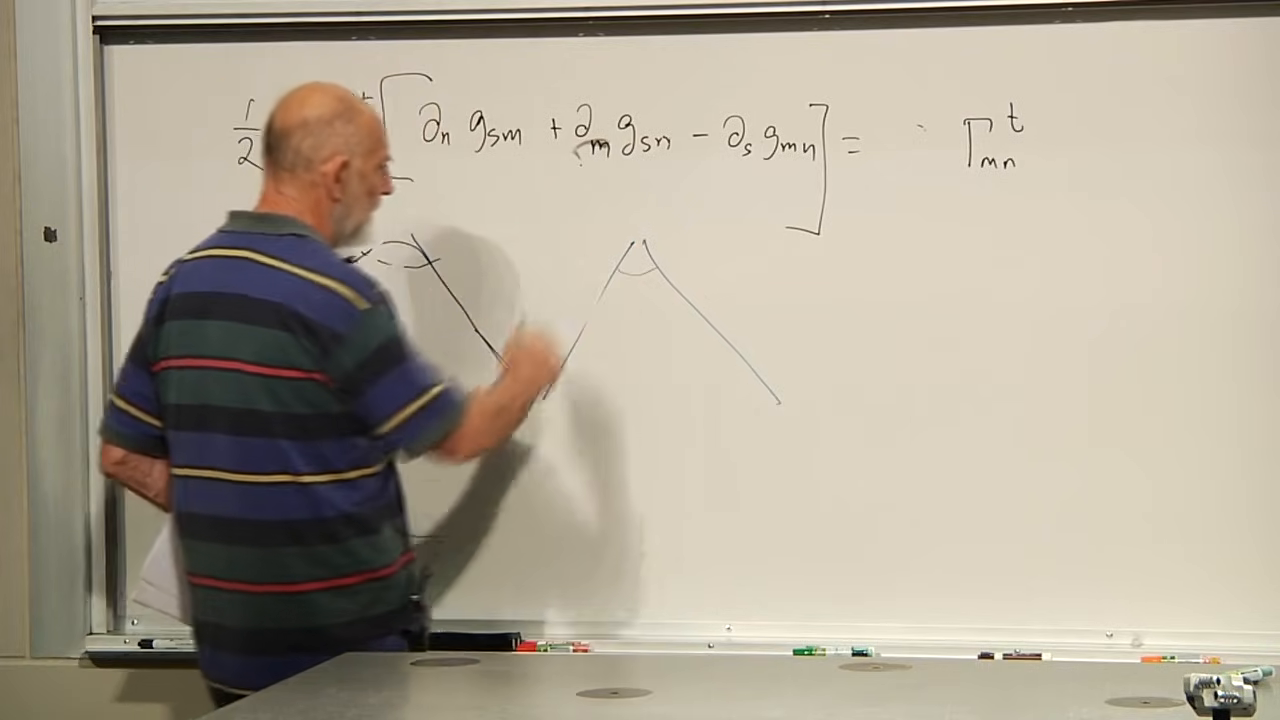
\includegraphics[width=\linewidth]{lecture_03_figure_21.png}
\caption{引入的圆锥作为一种几何：在远离其尖端处局部平坦，但在尖端集中了非平凡的曲率。}
\lectureframe{01:23:00}
\end{figure}

\begin{figure}[H]
\centering
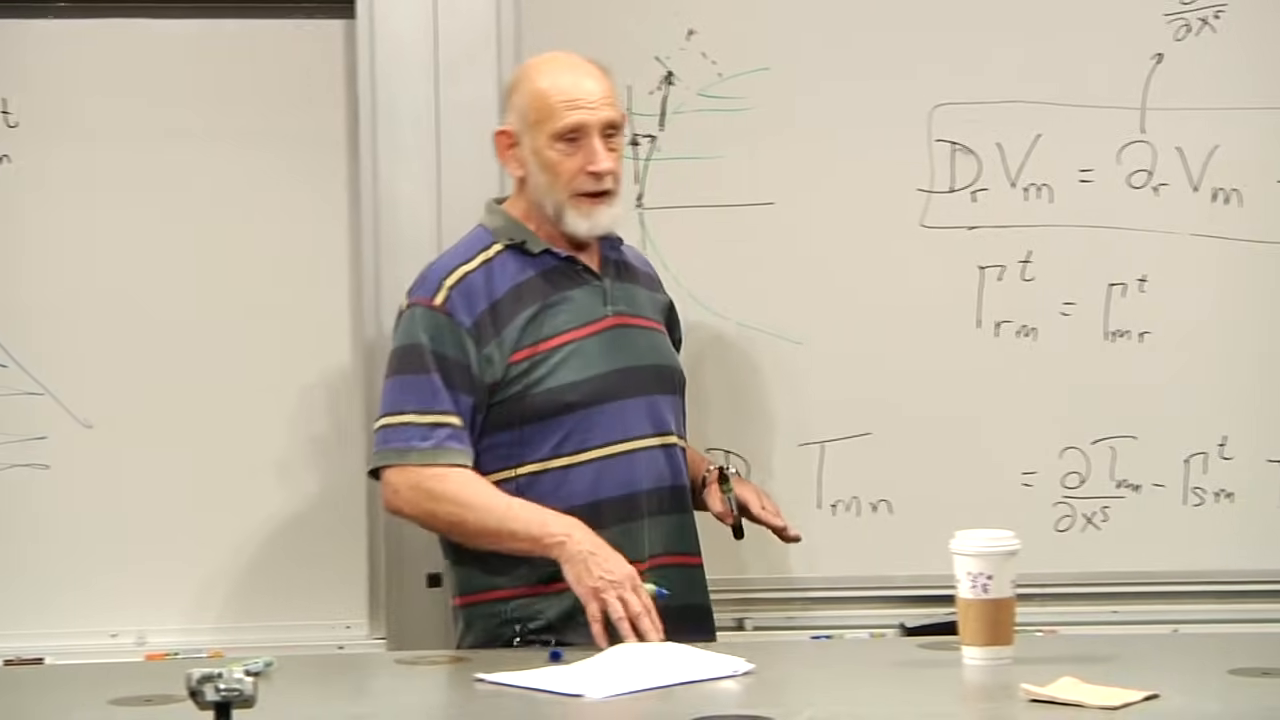
\includegraphics[width=\linewidth]{lecture_03_figure_22.png}
\caption{从圆盘上切下一个楔形并认同其边缘，产生圆锥亏角。}
\lectureframe{01:24:20}
\end{figure}

纸的构造使这一区分变得具体可感。在剪开的纸片上，沿普通平面中的平行方向平移一个矢量。在楔形边缘被认同之后，一条环绕尖端的路径回到起点时，被平移的矢量相对于其初始方向发生了旋转。

\begin{figure}[H]
\centering
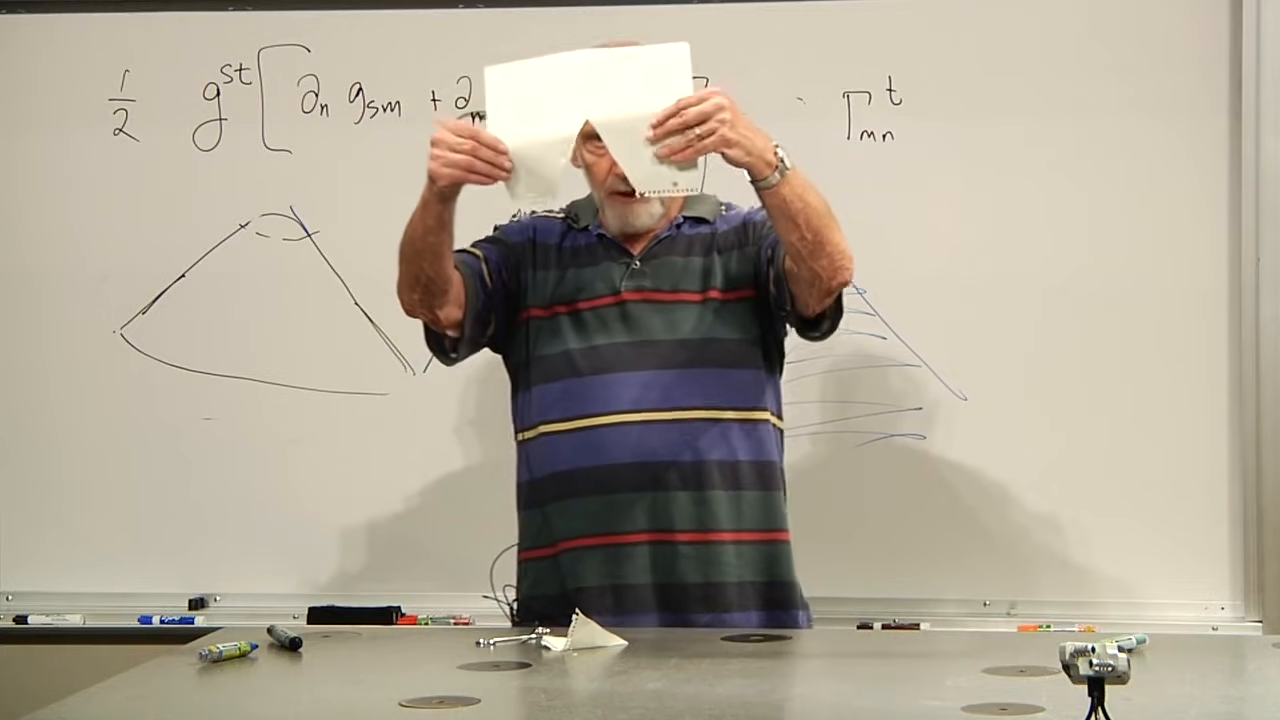
\includegraphics[width=0.78\linewidth]{lecture_03_figure_23.png}
\caption{纸锥演示：一张去掉楔形的平坦纸片，当其剪开的边缘被粘合时变成一个圆锥。}
\lectureframe{01:25:10}
\end{figure}

\begin{figure}[H]
\centering
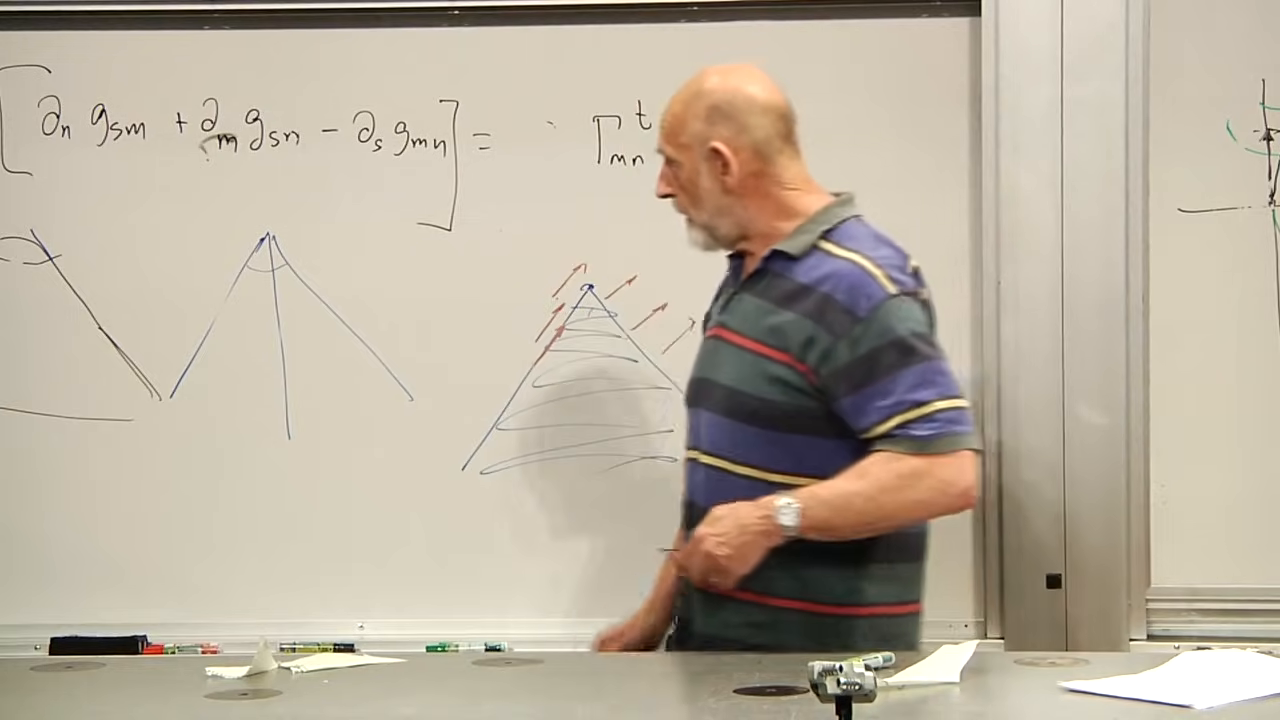
\includegraphics[width=\linewidth]{lecture_03_figure_24.png}
\caption{在边缘被认同之前，画在剪开的楔形上的矢量。}
\lectureframe{01:27:40}
\end{figure}

这种旋转就是和乐。它不是由沿某一段的坐标选择不当造成的。每一小段都可以在局部平坦的标架中处理。只有当这些局部比较绕一个闭合回路复合起来之后，效应才显现出来。对于理想圆锥，净旋转等于亏角，至多相差一个定向。

\begin{figure}[H]
\centering
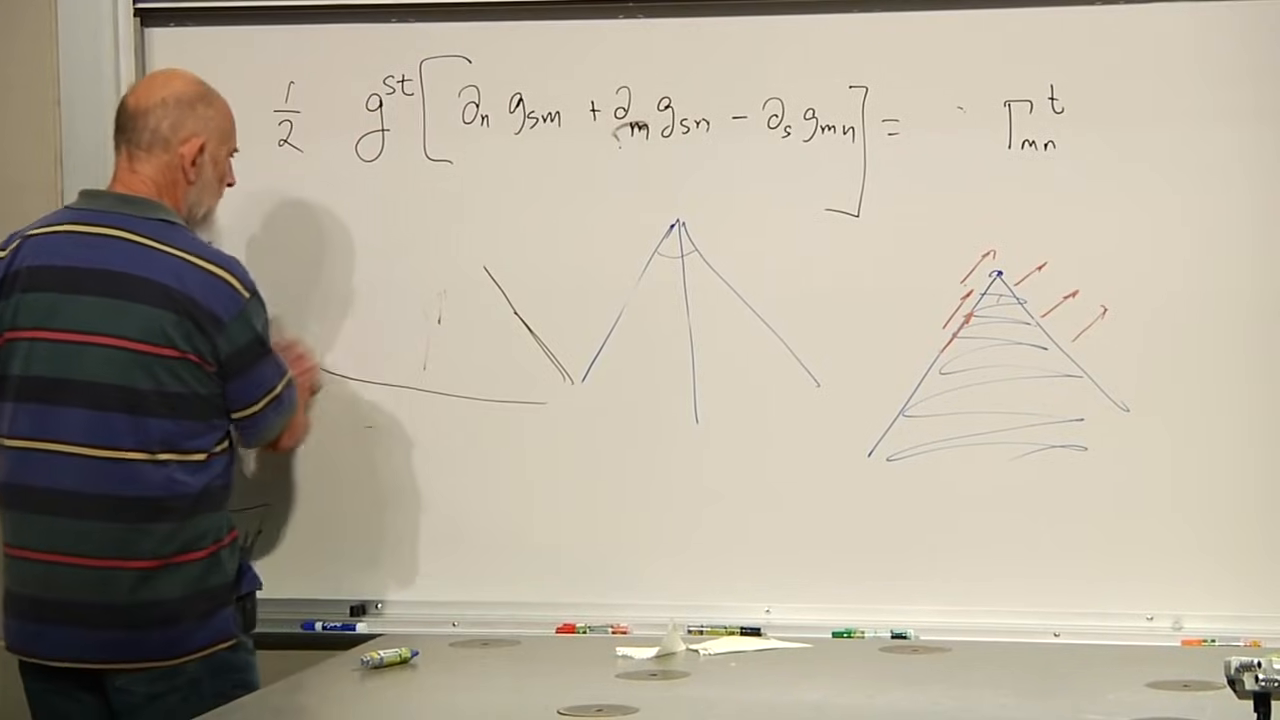
\includegraphics[width=\linewidth]{lecture_03_figure_25.png}
\caption{绕圆锥尖端平行移动返回的矢量方向发生了旋转：和乐记录了所包围的曲率。}
\lectureframe{01:29:10}
\end{figure}

\section{绕无穷小回路的两条路径}

把有限回路换成微小的坐标矩形。从一个角出发，先沿\(r\)方向平移，再沿\(s\)方向平移。把这一结果与先沿\(s\)再沿\(r\)平移的结果相比较。在平坦的笛卡儿坐标中，两条路径一致。在弯曲几何中，它们一般不一致。

\begin{figure}[H]
\centering
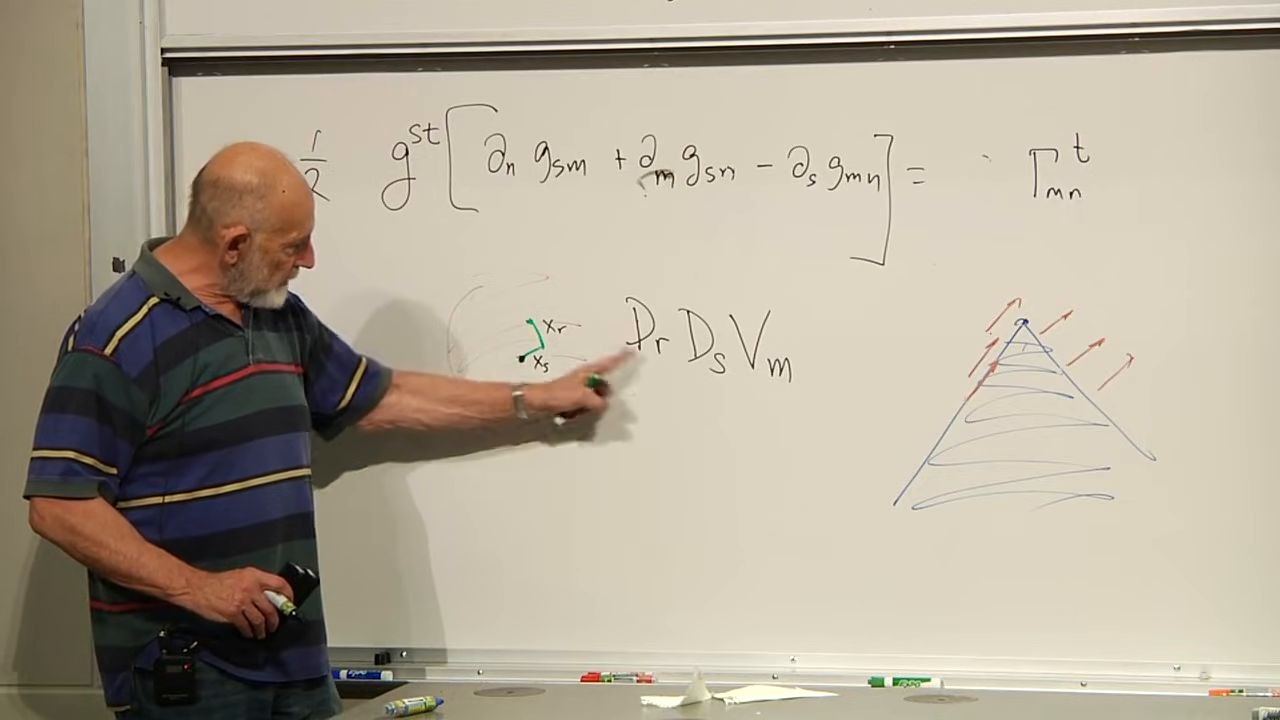
\includegraphics[width=\linewidth]{lecture_03_figure_26.png}
\caption{绕坐标矩形的无穷小平移的两种次序。}
\lectureframe{01:31:40}
\end{figure}

其代数度量是协变导数的对易子：
\begin{equation}
 \left(\nabla_s\nabla_r-\nabla_r\nabla_s\right)V_n.
\label{eq:l3-commutator}
\end{equation}
普通的混合偏导数在光滑函数上是对易的。这里的失败来自既要对矢量分量求导，也要对联络项求导。

\begin{figure}[H]
\centering
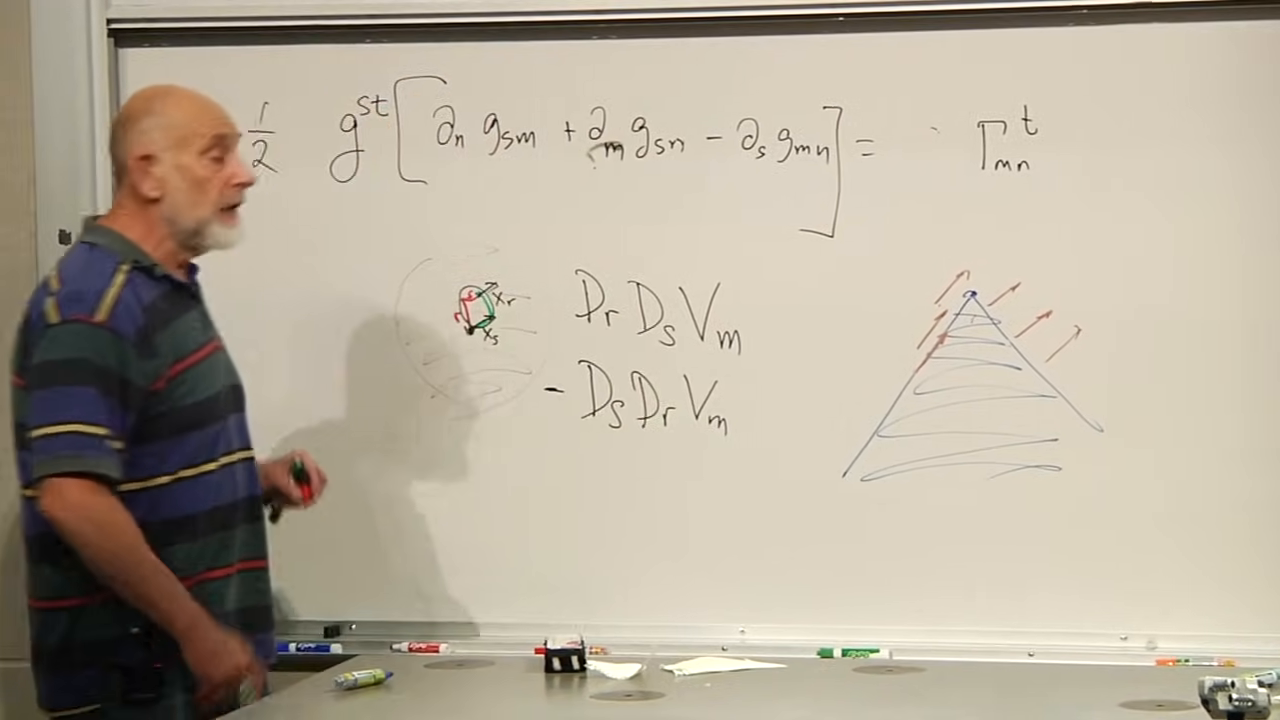
\includegraphics[width=\linewidth]{lecture_03_figure_27.png}
\caption{由协变微分的两种次序之差所表示的无穷小回路。}
\lectureframe{01:33:20}
\end{figure}

要计算它，首先把
\[
 T_{rn}=\nabla_rV_n
\]
看作一个二阶协变张量。然后用
\eqref{eq:l3-rank-two-derivative}沿\(s\)方向对\(T_{rn}\)求导。把\(r\)与\(s\)互换后重复，再相减。这一运算冗长但机械：展开、应用乘积法则，并消去含有\(V_n\)的二阶偏导数的项。

\begin{figure}[H]
\centering
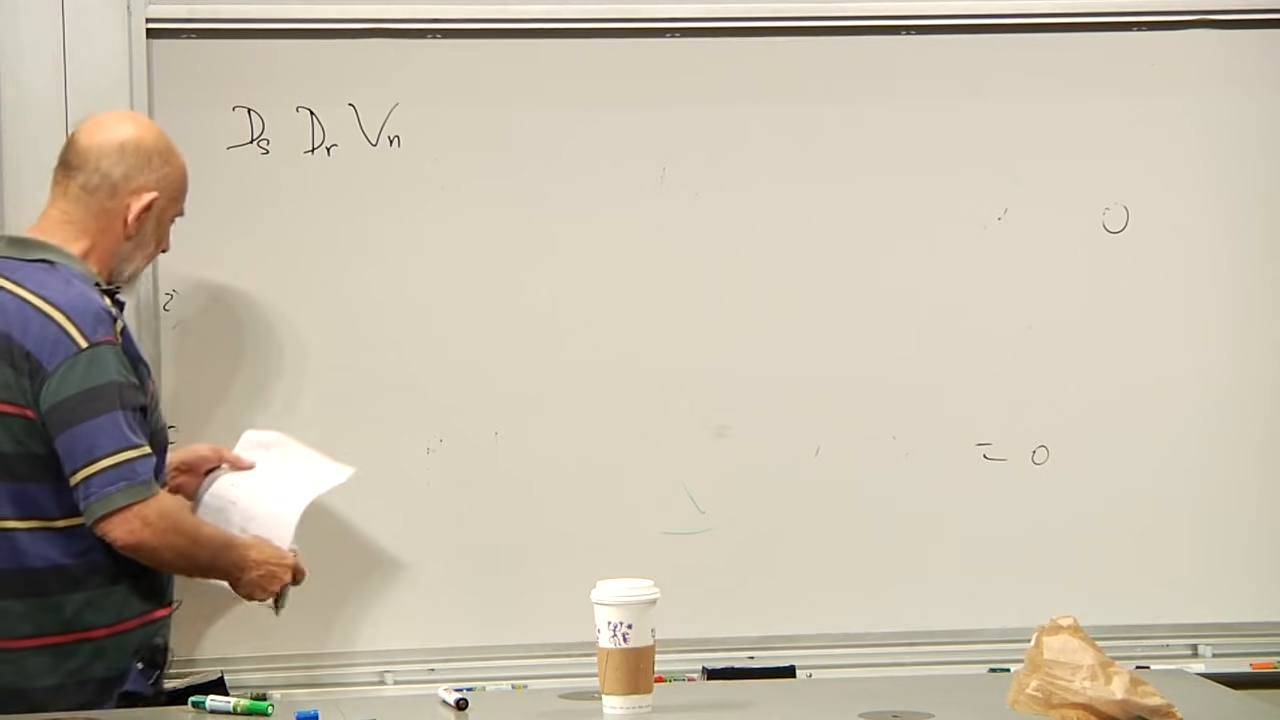
\includegraphics[width=\linewidth]{lecture_03_figure_28.png}
\caption{通过把\(\nabla_rV_n\)当作二阶张量来开始二重协变导数。}
\lectureframe{01:35:40}
\end{figure}

采用黑板上所取的约定，结果是
\begin{equation}
 \left(\nabla_s\nabla_r-\nabla_r\nabla_s\right)V_n
 =R_{srn}{}^tV_t.
\label{eq:l3-riemann-commutator}
\end{equation}

\begin{figure}[H]
\centering
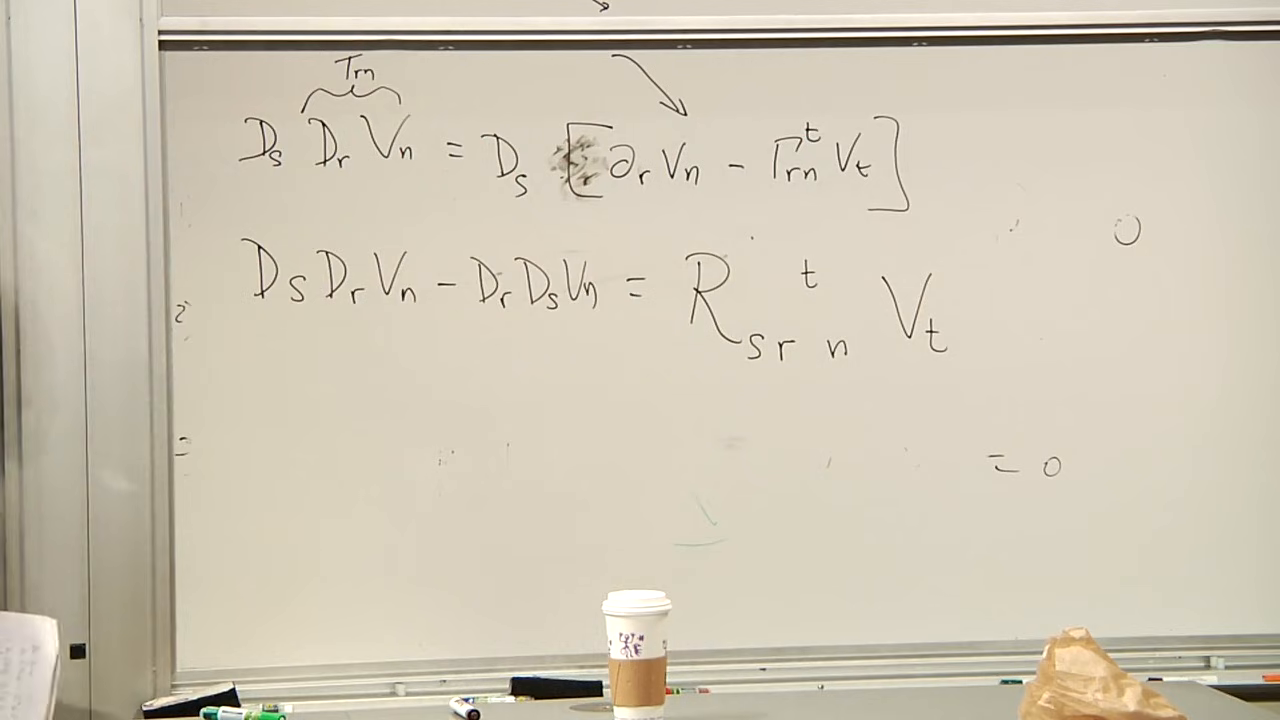
\includegraphics[width=\linewidth]{lecture_03_figure_29.png}
\caption{协变导数的对易子定义了曲率张量对一个余矢量的作用。}
\lectureframe{01:38:30}
\end{figure}

对于对易子的这种次序，
\begin{equation}
\begin{split}
 R_{srn}{}^t
={}&
 \partial_r\Gamma^t{}_{sn}
 -\partial_s\Gamma^t{}_{rn}\\
&+\Gamma^p{}_{sn}\Gamma^t{}_{pr}
 -\Gamma^p{}_{rn}\Gamma^t{}_{ps}.
\end{split}
\label{eq:l3-riemann}
\end{equation}
其他文本可能把符号反过来或把指标排列得不同；约定通过同时写出
\eqref{eq:l3-riemann-commutator}和\eqref{eq:l3-riemann}来固定。

\begin{figure}[H]
\centering
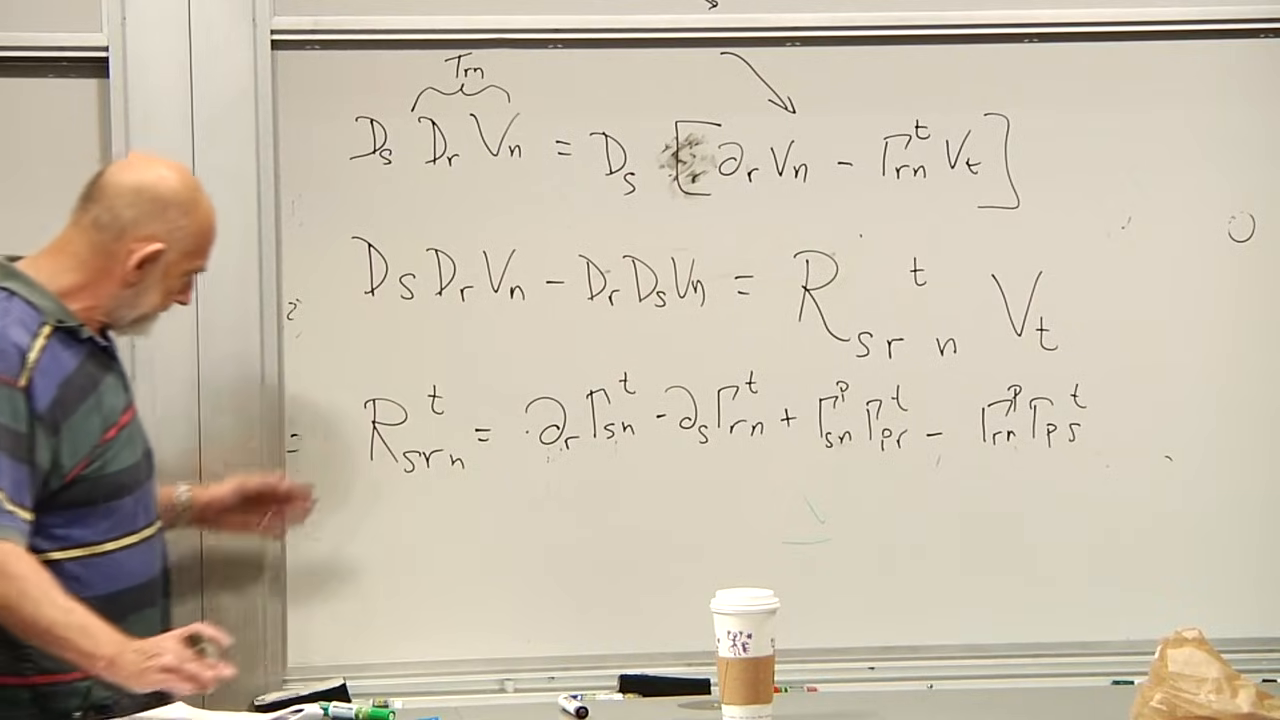
\includegraphics[width=\linewidth]{lecture_03_figure_30.png}
\caption{黎曼张量：联络的两个导数和两个二次联络项。}
\lectureframe{01:39:40}
\end{figure}

方程\eqref{eq:l3-christoffel}说明了为什么曲率首次出现在度规的二阶项中。每个\(\Gamma\)都包含\(g\)的一阶导数。因此，\eqref{eq:l3-riemann}中的导数项包含\(g\)的二阶导数，而二次项则包含一阶导数的乘积。在\(P\)处的法坐标中，联络本身为零，但其导数一般不为零，因此曲率仍然存在：
\[
\begin{aligned}
 \Gamma^t{}_{mn}(P)&=0,\\
 R_{srn}{}^t(P)
 &=\partial_r\Gamma^t{}_{sn}(P)
 -\partial_s\Gamma^t{}_{rn}(P).
\end{aligned}
\]
重要的是要理清导数的阶数：黎曼张量使用\(\Gamma\)的一阶导数，而它们相对于度规是二阶的。

这就是所需的诊断方法。如果黎曼张量的每个分量在整个区域内都为零，那么该区域就是局部平坦的。如果任何分量在某一点不为零，那么任何坐标变换都无法消除该处的曲率。计算机代数系统可以从解析度规检验这些分量，但其概念无非是平行移动绕无穷小回路一周后无法闭合。

\section{曲率作为潮汐引力}

这种几何诊断具有直接的物理意义。想象一个由相连三角形构成的柔性物体。在平坦区域中，它可以无应力地移动。将它推入内禀度规弯曲的区域，连杆的不同部分无法全部保持其偏好的间距和角度。该物体必须拉伸、挤压或剪切。

\begin{figure}[H]
\centering
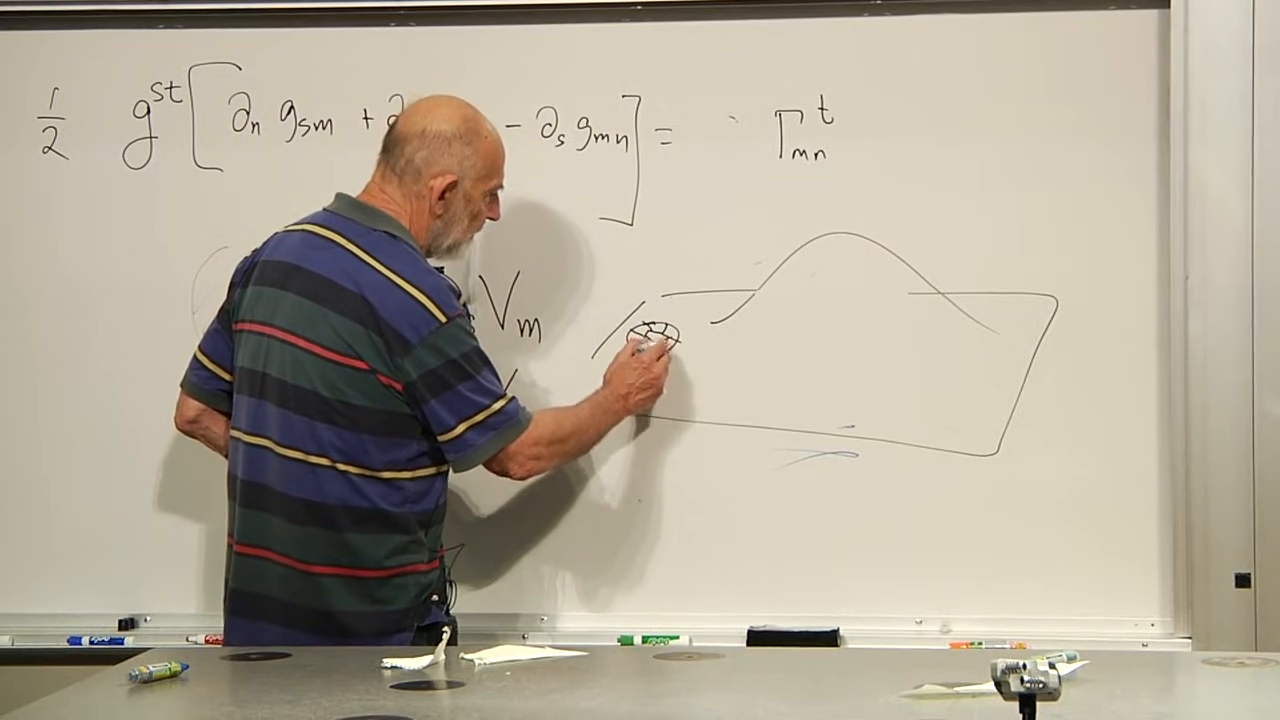
\includegraphics[width=\linewidth]{lecture_03_figure_31.png}
\caption{一个连杆物体从平坦区域移入弯曲隆起区域时，必须发生形变以跟随局部度规。}
\lectureframe{01:44:10}
\end{figure}

这种形变就是潮汐力的几何对应物。在引力场中，相邻的自由下落粒子可以相对彼此加速：一个方向可能被拉伸，而另一个方向被挤压。黎曼张量控制着这种相对加速度。在后来引入的测地偏离语言中，对于切矢量\(u^\mu\)和分离矢量\(\xi^\mu\)，
\begin{equation}
 \frac{D^2\xi^\mu}{D\tau^2}
 =-R^\mu{}_{\nu\rho\sigma}
 u^\nu\xi^\rho u^\sigma,
\label{eq:l3-geodesic-deviation-preview}
\end{equation}
其中整体符号取决于所选的曲率约定。这里不推导这个方程，但它精确地表达了讲座中的陈述：曲率和潮汐应力在字面上就是同一种局部物理。

一个理想的完全均匀引力场没有潮汐变化，并且可以通过过渡到匀加速参考系而在局部将其消除。由孤立质量产生的真实场并非完全均匀。地球的场近似沿径向指向，并随位置变化，因此相邻的自由下落轨迹会汇聚或分离。

\begin{figure}[H]
\centering
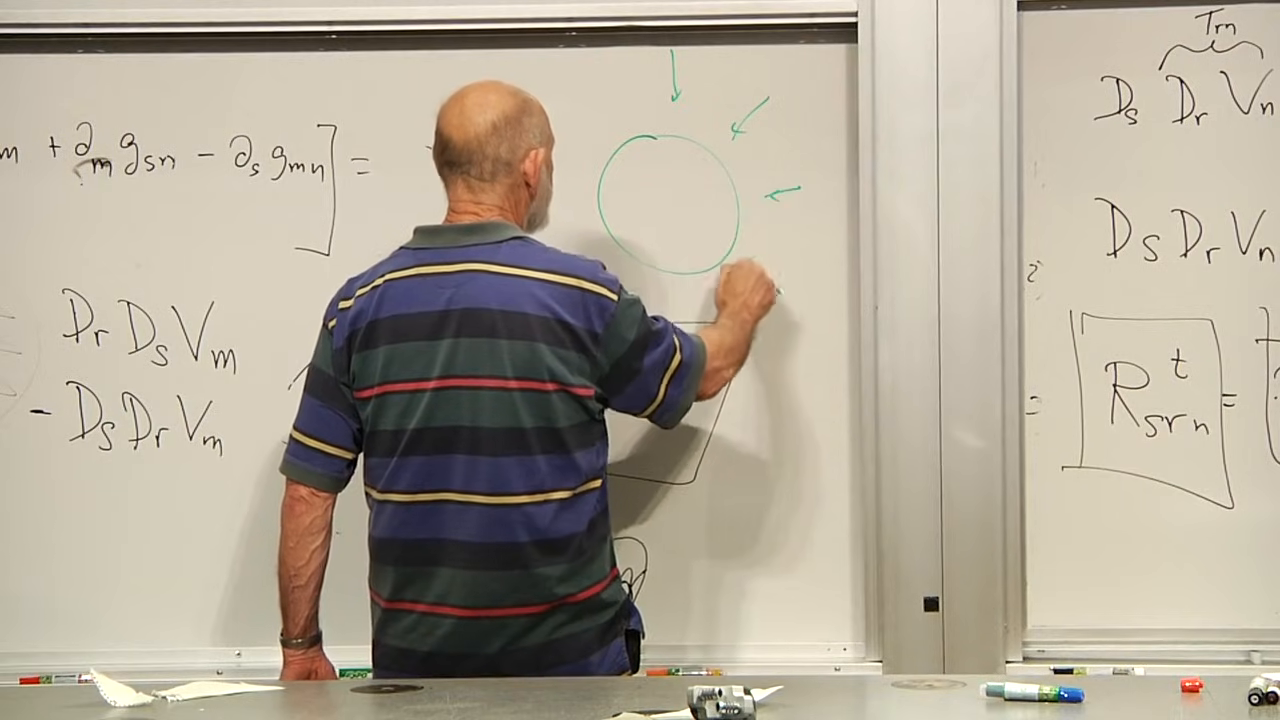
\includegraphics[width=\linewidth]{lecture_03_figure_32.png}
\caption{径向引力场在延展物体上发生变化，产生被认定为潮汐引力的相对加速度。}
\lectureframe{01:48:40}
\end{figure}

\begin{classroomqa}
\audiencequestion{是什么将真正的引力场与在加速参考系中看到的表观场区分开来？}
\lecturerresponse{匀加速参考系可以在局部实验中模仿均匀引力场，但它不会产生潮汐相对加速度。由真实物质产生的场会随位置变化，因此会产生潮汐力。这些力是不变的证据，表明该效应不仅仅是一种坐标变换。一个完全均匀的真实场是一种理想化；在大物体表面足够小的一块区域附近，实际场只能近似均匀。\lecturetimestamp{01:46:54}}
\end{classroomqa}

\begin{classroomqa}
\audiencequestion{为什么下落物体的大小对潮汐效应很重要？}
\lecturerresponse{曲率比较的是相邻位置。一个远小于场变化长度尺度的物体，其各部分几乎感受到相同的加速度，因此几乎不发生形变。一个延展物体则感受到更大的差异。地球附近一个自由下落的细菌感受到的潮汐应力可以忽略不计，而讲座中假想的两千英里高的人则会受到严重扭曲。曲率具有局部值，但累积的形变与所比较的分离尺度成比例。
\lecturetimestamp{01:49:01}}
\end{classroomqa}

\begin{classroomqa}
\audiencequestion{如果平坦性要求检查每一点的曲率，这个检验是否仍然是一个无限的问题？}
\lecturerresponse{对于以解析形式给出的度规，导数和曲率分量都是解析表达式。人们将它们作为位置的函数计算一次，通常就能看出它们是否恒为零。如果度规仅以数值表的形式给出，那么就必须在整个采样区域内估计并检查曲率，这确实可能代价高昂。即便如此，这也比在每一点搜索所有可能的坐标系要明确得多。
\lecturetimestamp{01:50:37}}
\end{classroomqa}

\section{已经确立的内容}

现在可以把这一论证读作一条连续的链条：
\begin{enumerate}
 \item 在任意选定的点，坐标可以使得
 \(g_{mn}=\delta_{mn}\) 和 \(\partial_rg_{mn}=0\)。
 \item 张量分量的普通导数不能像张量那样变换，因为坐标基逐点变化。
 \item 联络修正了这种基的变化，并定义了协变微分。
 \item 度规兼容性和零挠率从度规唯一地确定联络。
 \item 两个协变导数的不对易由黎曼张量给出。这种不对易度量了和乐、度规的二阶变化以及潮汐引力。
\end{enumerate}

因此，所承诺的曲率诊断量已经在不选择任何特殊全局坐标系的情况下构造出来了。下一步是从正定黎曼几何转向洛伦兹时空，把这些工具应用于恒星或黑洞的施瓦西几何，并回到本讲末尾所推迟的测地线。